%% 
%% Copyright 2007-2020 Elsevier Ltd
%% 
%% This file is part of the 'Elsarticle Bundle'.
%% ---------------------------------------------
%% 
%% It may be distributed under the conditions of the LaTeX Project Public
%% License, either version 1.2 of this license or (at your option) any
%% later version.  The latest version of this license is in
%%    http://www.latex-project.org/lppl.txt
%% and version 1.2 or later is part of all distributions of LaTeX
%% version 1999/12/01 or later.
%% 
%% The list of all files belonging to the 'Elsarticle Bundle' is
%% given in the file `manifest.txt'.
%% 

%% Template article for Elsevier's document class `elsarticle'
%% with numbered style bibliographic references
%% SP 2008/03/01
%%
%% 
%%
%% $Id: elsarticle-template-num.tex 190 2020-11-23 11:12:32Z rishi $
%%
%%
%%\documentclass[preprint,12pt]{elsarticle}

%% Use the option review to obtain double line spacing
%% \documentclass[authoryear,preprint,review,12pt]{elsarticle}

%% Use the options 1p,twocolumn; 3p; 3p,twocolumn; 5p; or 5p,twocolumn
%% for a journal layout:
%% \documentclass[final,1p,times]{elsarticle}
%% \documentclass[final,1p,times,twocolumn]{elsarticle}
%% \documentclass[final,3p,times]{elsarticle}
 \documentclass[final,3p,times,twocolumn]{elsarticle}
%% \documentclass[final,5p,times]{elsarticle}
%% \documentclass[final,5p,times,twocolumn]{elsarticle}

%% For including figures, graphicx.sty has been loaded in
%% elsarticle.cls. If you prefer to use the old commands
%% please give \usepackage{epsfig}

%% The amssymb package provides various useful mathematical symbols
\usepackage{amssymb}
\usepackage{nicefrac}
\usepackage{booktabs}  % Para líneas mejoradas en tablas
\usepackage{multirow}  % Para combinar filas si es necesario
\usepackage{tikz}      % Para dibujar los triángulos
\usepackage{subcaption}   % Para las subfiguras
\usepackage{url} % o \usepackage{hyperref}
%\usepackage{cite}

\newcommand{\triangleup}[1][black]{%
    \tikz\draw[fill=#1] (0,0) -- (0.2,0) -- (0.1,0.2) -- cycle;%
}
% Comando personalizado para cuadrados
\newcommand{\squarecolor}[1][black]{%
    \tikz\draw[fill=#1] (0,0) rectangle (0.2,0.2);%
}
%% The amsthm package provides extended theorem environments
%% \usepackage{amsthm}

%% The lineno packages adds line numbers. Start line numbering with
%% \begin{linenumbers}, end it with \end{linenumbers}. Or switch it on
%% for the whole article with \linenumbers.
%% \usepackage{lineno}

\journal{Sensors and Actuators B: Chemical}

\begin{document}

\begin{frontmatter}

%% Title, authors and addresses

%% use the tnoteref command within \title for footnotes;
%% use the tnotetext command for theassociated footnote;
%% use the fnref command within \author or \address for footnotes;
%% use the fntext command for theassociated footnote;
%% use the corref command within \author for corresponding author footnotes;
%% use the cortext command for theassociated footnote;
%% use the ead command for the email address,
%% and the form \ead[url] for the home page:
%% \title{Title\tnoteref{label1}}
%% \tnotetext[label1]{}
%% \author{Name\corref{cor1}\fnref{label2}}
%% \ead{email address}
%% \ead[url]{home page}
%% \fntext[label2]{}
%% \cortext[cor1]{}
%% \affiliation{organization={},
%%             addressline={},
%%             city={},
%%             postcode={},
%%             state={},
%%             country={}}
%% \fntext[label3]{}

%\title{Optimized Instrumental Odour Monitoring System for Onboarded Applications}

%\title{New Application of Nested Sequential Forward Feature Selection: Optimizing Instrumental Odour Monitoring Systems in Drones}
\title{Informed Feature Selection Algorithm for Optimizing Instrumental Odour Monitoring Systems in Drones}
%% use optional labels to link authors explicitly to addresses:
%% \author[label1,label2]{}
%% \affiliation[label1]{organization={},
%%             addressline={},
%%             city={},
%%             postcode={},
%%             state={},
%%             country={}}
%%
%% \affiliation[label2]{organization={},
%%             addressline={},
%%             city={},
%%             postcode={},
%%             state={},
%%             country={}}


\author[IBEC]{Alessandro Benegiamo}
\author[UB]{Javier Alonso-Valdesueiro*}
\author[UB]{Javier Burgues}
\author[IBEC]{Albert Vidal}
\author[UB]{Agustin Gutierrez-Galvez}
\author[UB,IBEC]{Santiago Marco}

\affiliation[UB]{organization={Department of Electronic and Biomedical Engineering, University of Barcelona},%Department and Organization
            addressline={Martí i Franquès 1,}, 
            city={Barcelona},
            postcode={08028}, 
            state={Catalonia},
            country={Spain}}

\affiliation[IBEC]{organization={Signal and Information Processing for Sensing Systems Group, Institute for Bioengineering of Catalonia},%Department and Organization
            addressline={Baldiri i Reixac, 4 Torre I}, 
            city={Barcelona},
            postcode={08028}, 
            state={Catalonia},
            country={Spain}}

\begin{abstract}
%% Text of abstract
%%This study aims to present a new application of the Nested Sequential Forward Feature Selection algorithm when applying to optimize the performance of Instrumental Odour Monitoring Systems on-boarded in drones. When combined with The Interval Partial Least Square Regression model (the NiPLS algorithm), it reduces the Root Mean Square error of prediction (RMSEP) and the Limits of Agreement (LoA) at 95\% Confident Interval (CI) compared with traditional approaches in Feature selection and Cross Validation of the model. The algorithm is applied twice, first for selecting the most relevant sensors and then, for selecting the most relevant period of acquisition. This optimization procedure was tested on data obtained from the IOMS onboarded in an octocopter drone flying over a Waste Water Treatment Plant (WWTP). The RMSEP reduced from 2.1x to 1.8x and maximum LoA at $95$\% CI reduces from 5x to 3.4x with correlation coefficient of \~0.9 when measurements were taken from different sources in a particular WWTP.


This study demonstrates how advanced feature selection significantly enhances the performance of Instrumental Odour Monitoring Systems (IOMS) on-boarded in drones. By employing the Nested Sequential Forward Feature Selection algorithm in conjunction with the Interval Partial Least Squares (NiPLS) regression model, a notable reductions in the Root Mean Square Error of Prediction (RMSEP) and the Limits of Agreement (LoA) at a 95\% Confidence Interval (CI) are achievied during test of the quantification model. The feature selection process is applied in two stages: first, to identify the most relevant sensors, and second, to determine the optimal acquisition periods. This method was validated using data from an IOMS mounted on an octocopter drone over a Wastewater Treatment Plant (WWTP). Results show a reduction in RMSEP from 2.1x to 1.8x and a decrease in maximum LoA at 95\% CI from 5x to 3.4x, with a correlation coefficient of approximately 0.9 for measurements from various sources within a particular WWTP.
\end{abstract}

%%Graphical abstract
%\begin{graphicalabstract}
%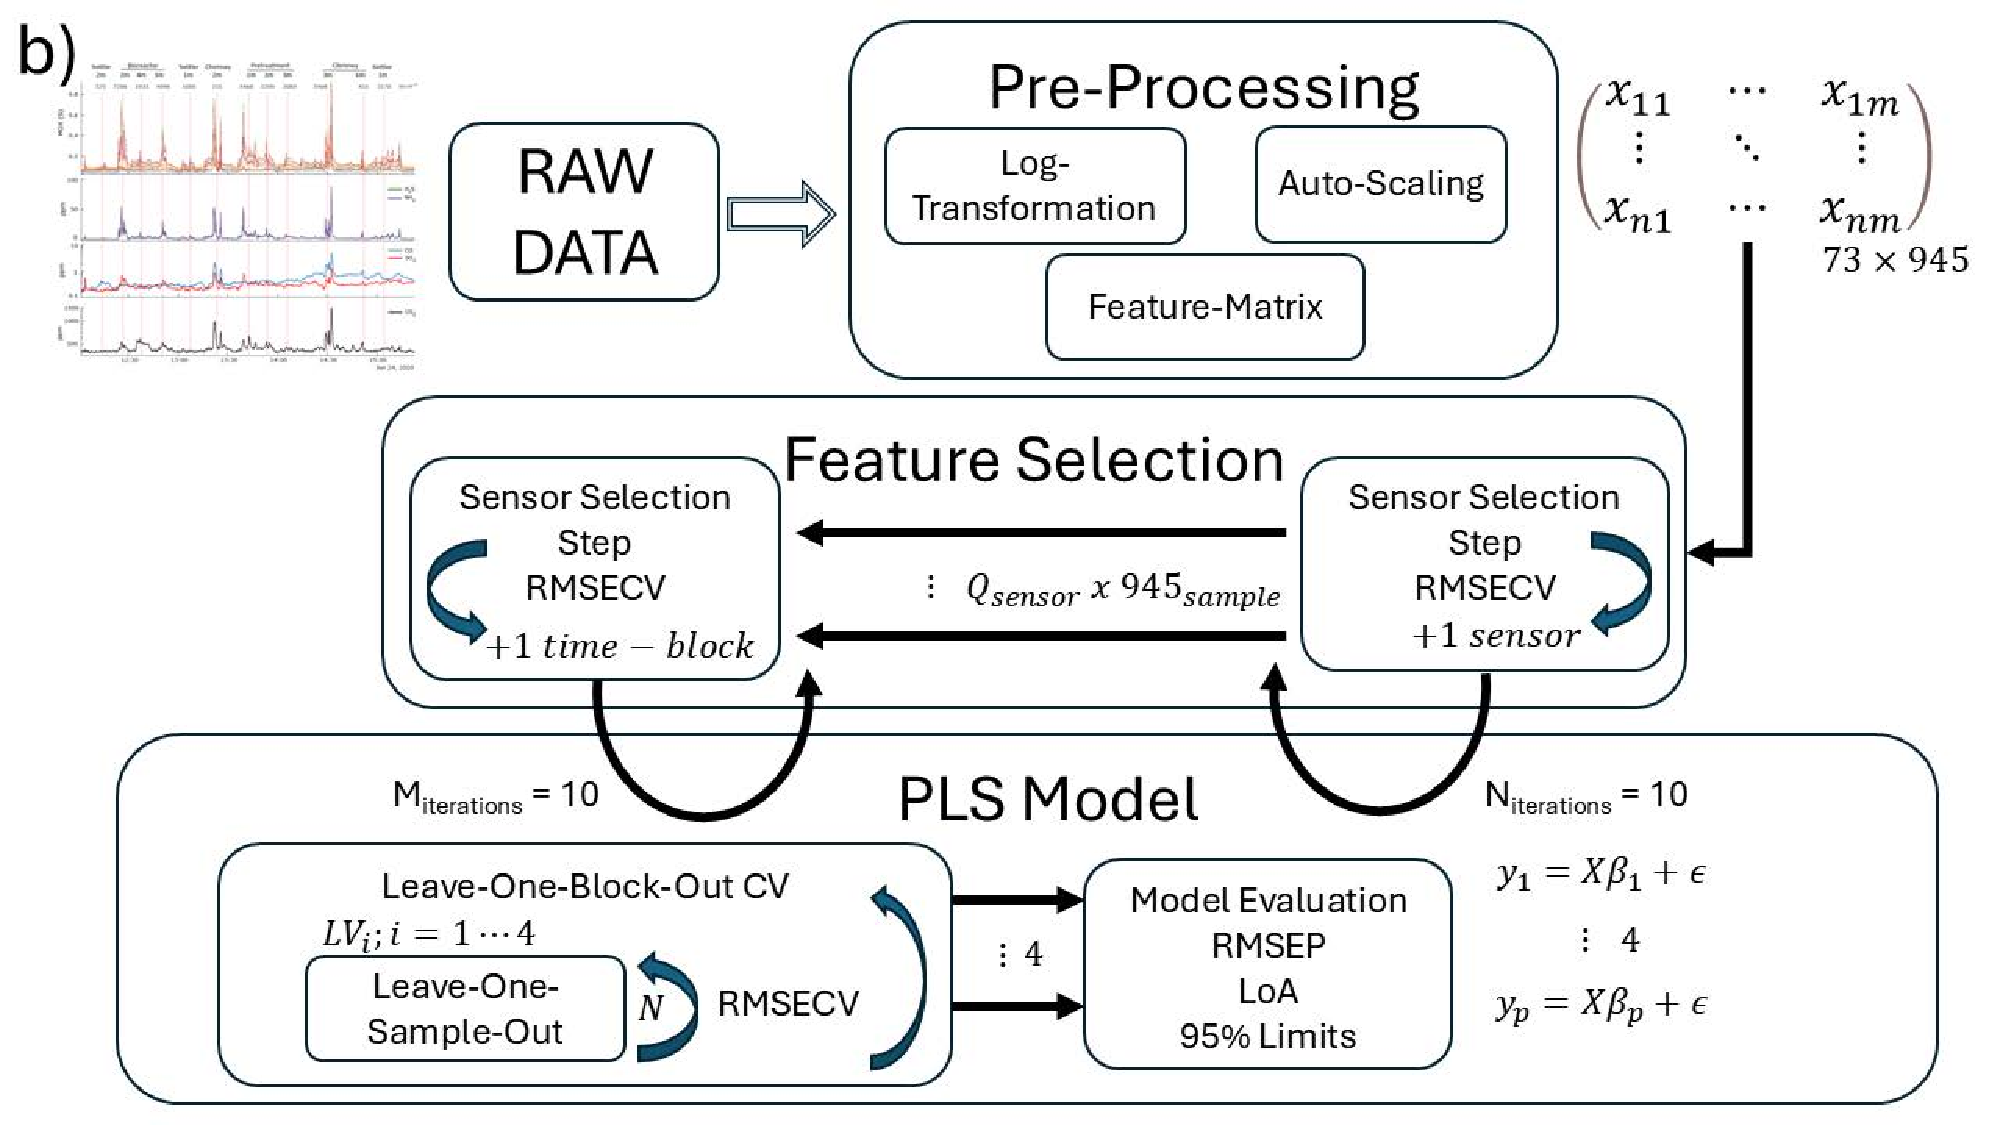
\includegraphics[width=\textwidth]{fig4b.pdf}
%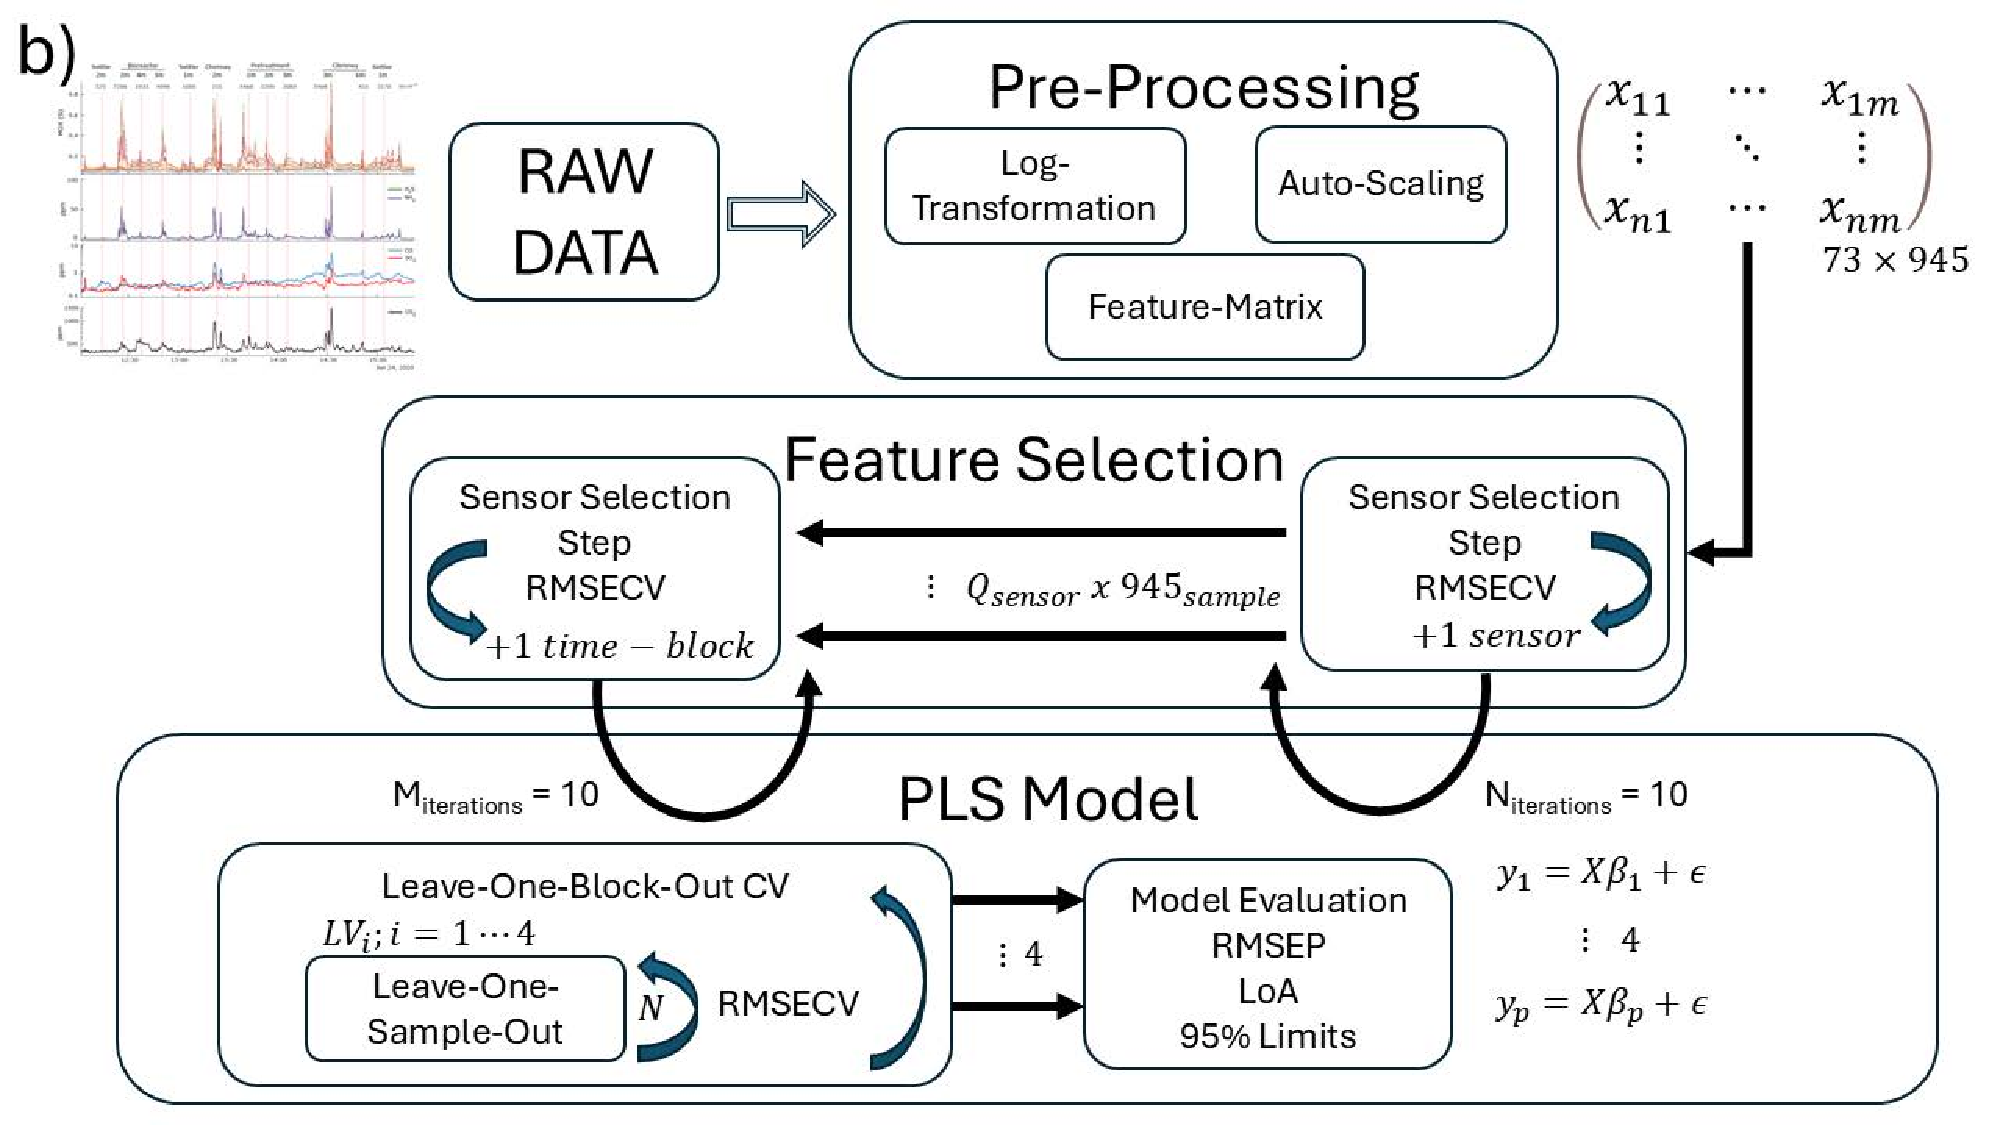
\includegraphics{fig4b.pdf}
%\end{graphicalabstract}

%%Research highlights
%\begin{highlights}
%\item Research highlight 1
%\item Research highlight 2
%\end{highlights}

\begin{keyword}
%% keywords here, in the form: keyword \sep keyword
Instrumental Odour Monitoring System  \sep Chemical sensors  \sep Feature selection  \sep Odour quantification  \sep On-boarded system \sep Drone Instrumentation
%% PACS codes here, in the form: \PACS code \sep code
%%\PACS 0000 \sep 1111
%% MSC codes here, in the form: \MSC code \sep code
%% or \MSC[2008] code \sep code (2000 is the default)
%%\MSC 0000 \sep 1111
\end{keyword}

\end{frontmatter}

%% \linenumbers

%% main text
\section{Introduction}
\label{sec:intro}

%%Odour quantification in industrial environments have recently attracted attention due to legal regulation in modern countries \cite{Brinkmann2018,TotalG,Zhou2019}. Governments have established regulation on measurement methods and permitted levels of odour in different situations \cite{Scentroid}. The most extended method for odour quantification is the dynamic olfactometry, where a human panel determines the level of odour when exposed to a sample of air \cite{Sironi2010}.  The air is taken from the industrial environment under study in sampling bags, diluted at different concentrations and delivered to the human panel for quantifications. Despite its extended use and legal endorsement, odour quantification using dynamic olfactometry presents several problems that reduces its applicability. First, it presents a Limit of Agreement (LoA) of 2x with a Confident Interval (CI) of 95\% in every quantification [ref]. Second, it only allows punctual pool of the industrial environment. And finally, a full characterization of the odour coming from an industrial plant might scale in budget quite fast.

%%For these reasons, in the last decades, Instrumental Our Monitoring Systems (IOMSs) have been deployed as odour quantification tools in industrial environments \cite{cangialosi2018}. In particular, their deployment in Wastewater Treatment Plants (WWTPs) have demonstrated to be a very useful tool for plant managers regarding adjust the odour levels to the legal regulation \cite{Capelli2008}. Furthermore, new designs which consist in on-boarded IOMS in drones, have been developed aiming 3D odour maps of WWTPs \cite{Burgues2020,Burgues2021_Ar}. When the IOMS is flying in a drone, the cost reduction by using IOMSs instead of odour characterization campaigns by dynamic olfactometries, reduces even further.  Within two days campaign, a characterization relevant odour emitters and a 3D odour map can be provided. Even, the odour quantification can be dynamically monitored, allowing the operator to choose where and when to sample. 

%%The on-boarded IOMS is typically equipped with an array of chemical sensors of different types and takes off with the drone. Flying over different odour sources in the plant, the IOMS measures the concentration of different gases in the air while sampling bags are filled. Once the measurements are done, dynamic olfactometries are performed using the sampling bags and an odour level in $\nicefrac{OU_{E}}{m^{3}}$ is provided for each source of the plant \cite{Burgues2020,Burgues2021,Burgues2021_Ar}. Therefore, each source is represented by a temporal series of measurements (one temporal series per sensor) or features and an odour level. Whit this information, the IOMS is calibrated using multivariate prediction models. The models are trained with the data from the sensor array and the dynamic olfactometries and, afterwards, the model quantifies the odour by observing the signals coming from the sensor array. 


%Partial Least Squares (PLS) \cite{Wold1984} is the most common multivariate model to predict odour concentration in the field \cite{Capelli2008,Burgues2021}. Particularly well suited for datasets with time series and few samples, its performance can be improved by reducing the features in each sample by different reduction methods. In the field of on-boarded IOMSs, the Variable Importance in Projection (VIP) method \cite{Chong2005} has become the most extended feature reduction method. 

%%In this method, VIPs scores are calculated as the squares of the PLS weights provide information of the explained variance associated to each latent variable. Features with VIPs are selected following the “greater than one” rule for model optimisations, where a VIP score above 1 keeps the feature for future model training. Then, different techniques are applied for further elimination of data from the training dataset []. After this selection of features, the leave-one-block-out Cross Validation (CV) scheme \cite{Filzmoser2009} is commonly used for validation looking at the Root Mean Square Error of Cross Validation (RMSECV).

%%This procedure typically leads to RMSEP in the quantification of odour ~$2.3$x which in the worst-case scenario becomes a Limit of Agreement of $5$x with 95\% CI []. Therefore, the advantages of using on-boarded IOMSs in industrial plants get downsized by this poor performance and leave their use out of legal quality assessment or regulatory studies of the plants. In the last decade, a considerable amount of effort has been put on reduce the RMSEP of the model after CV by applying new algorithms able to work with datasets with small number of samples \cite{Hastie2009,Wold2001,Martens1989,Arlot2010}.

%%It is the aim of this contribution to present a new approach to this problem. Working with a small dataset obtained by an IOMS on-boarded in an DJI drone when flying over odour sources in a WWTP, the proposed solution is able to reduce the RMSEP and downsize the LoA at 95\% of CI by two points. A two step process for feature selection, based on the knowledge of the characteristics of the data collected by the IOMS, is presented.
%%It uses a Nested Sequential Forward Selection algorithm \cite{Jain1997,Saeys2007} in combination with Interval Partial Least Squares procedure \cite{Norgaard2000}. The process is applied twice, first for selecting the most relevant sensors and then, for selecting the most relevant period of acquisition.  
Odour quantification in industrial environments has gained attention due to legal regulations \cite{Brinkmann2018,TotalG,Zhou2019}. The most common method, dynamic olfactometry, involves a human panel that evaluates the odor levels of air samples \cite{Sironi2010}. However, this method has limitations, including a high Limit of Agreement (LoA) and significant costs.

Instrumental Odour Monitoring Systems (IOMSs) have been deployed as alternatives, particularly in Wastewater Treatment Plants (WWTPs) \cite{cangialosi2018,Capelli2008}. IOMSs onboard drones can create 3D odour maps and further reduce costs \cite{Burgues2020,Burgues2021_Ar}. These systems use chemical sensors to measure gas concentrations, and dynamic olfactometries are performed on collected samples to calibrate multivariate prediction models.

Partial Least Squares (PLS) \cite{Wold1984} is commonly used for odour prediction, with performance improved by feature reduction methods such as Variable Importance in Projection (VIP) \cite{Chong2005}. VIP scores help select relevant features for model training, followed by validation using Cross-Validation (CV) \cite{Filzmoser2009}.

Despite these methods, the Root Mean Square Error of Prediction (RMSEP) remains high, limiting the use of IOMSs for regulatory purposes. Recent efforts focus on reducing RMSEP with new algorithms for small datasets \cite{Hastie2009,Wold2001,Martens1989,Arlot2010}.

This paper presents a new approach that uses a small dataset from an IOMS onboard a DJI drone over a WWTP. A two-step feature selection process, combining Nested Sequential Forward Selection \cite{Jain1997,Saeys2007} and Interval Partial Least Squares \cite{Norgaard2000}, is proposed to improve model performance.

The presented contribution is organized as follows. Firstly, in the Methods section, the onboarded IOMS and the measurement campaign are presented. In this section, the data processing workflow is also described in detail. Secondly, in the Results and Discussion section, the performance figures of the proposed workflow are summarized when applied to the dataset obtained in the measurement campaign. Finally, in the Conclusions section, a summary of the NiPLS performance is presented, and its future applications in the field of onboarded IOMSs are described.  

\section{Methods}
\label{sec:methods}
\subsection{Onboarded IOMS}
\label{ssec:IOMS}
Fig.\ref{fig:ioms}(a) shows the block diagram of the onboarded IOMS performing measurements during flights. 
\begin{figure}[ht!]
    \centering
    % Primera subfigura
    \begin{subfigure}[b]{\columnwidth}
        \centering
        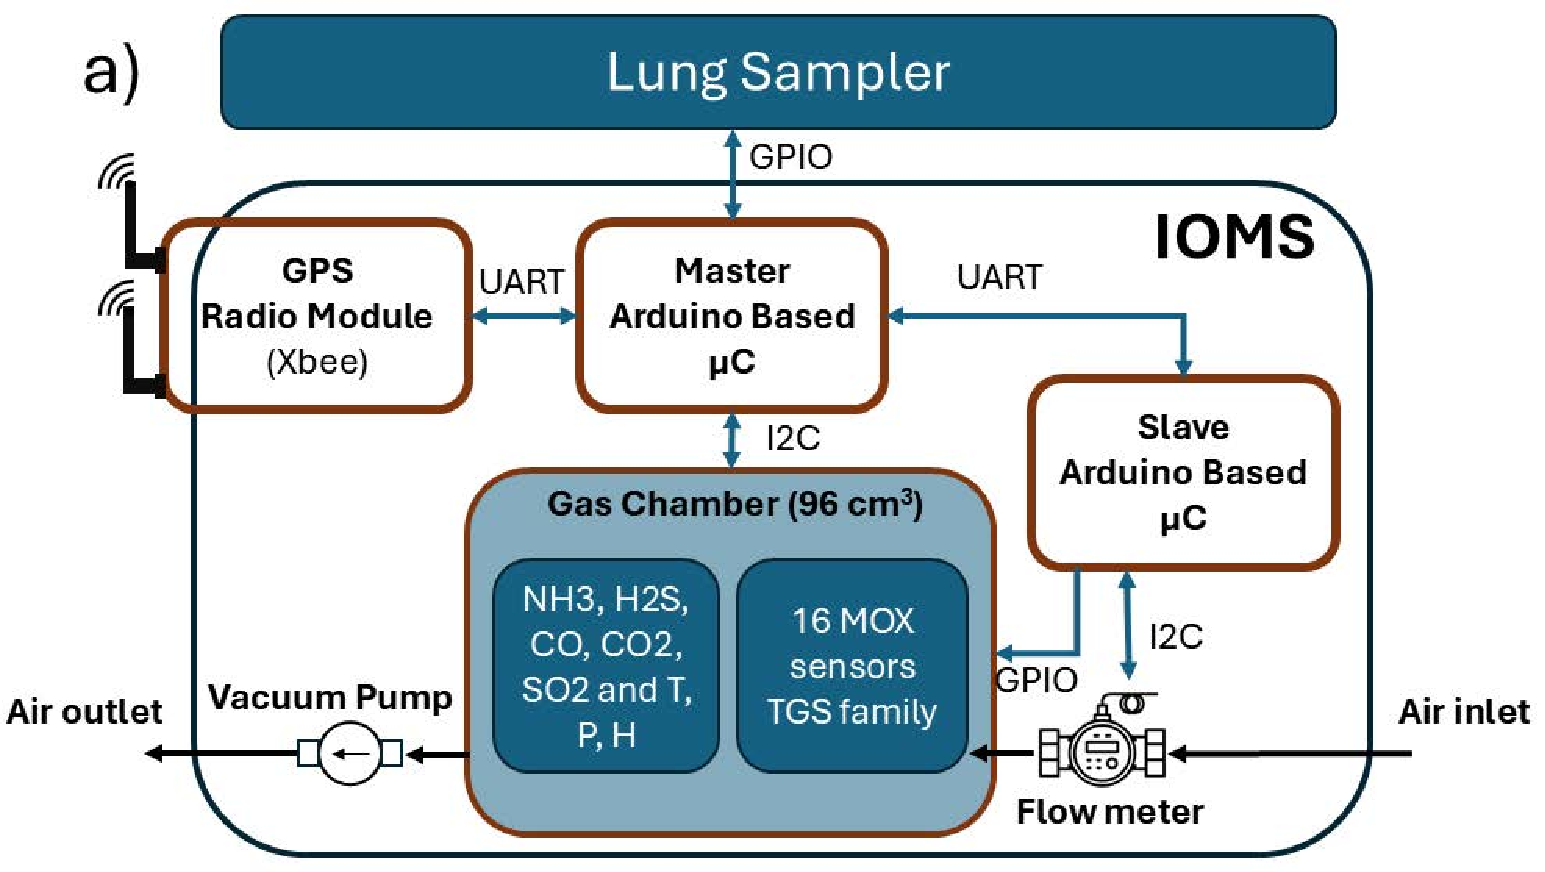
\includegraphics[width=\linewidth]{fig1a_2.pdf}
        \label{fig:ioms_a}
    \end{subfigure}
    
    % Segunda subfigura (la misma imagen)
    \begin{subfigure}[b]{\columnwidth}
        \centering
        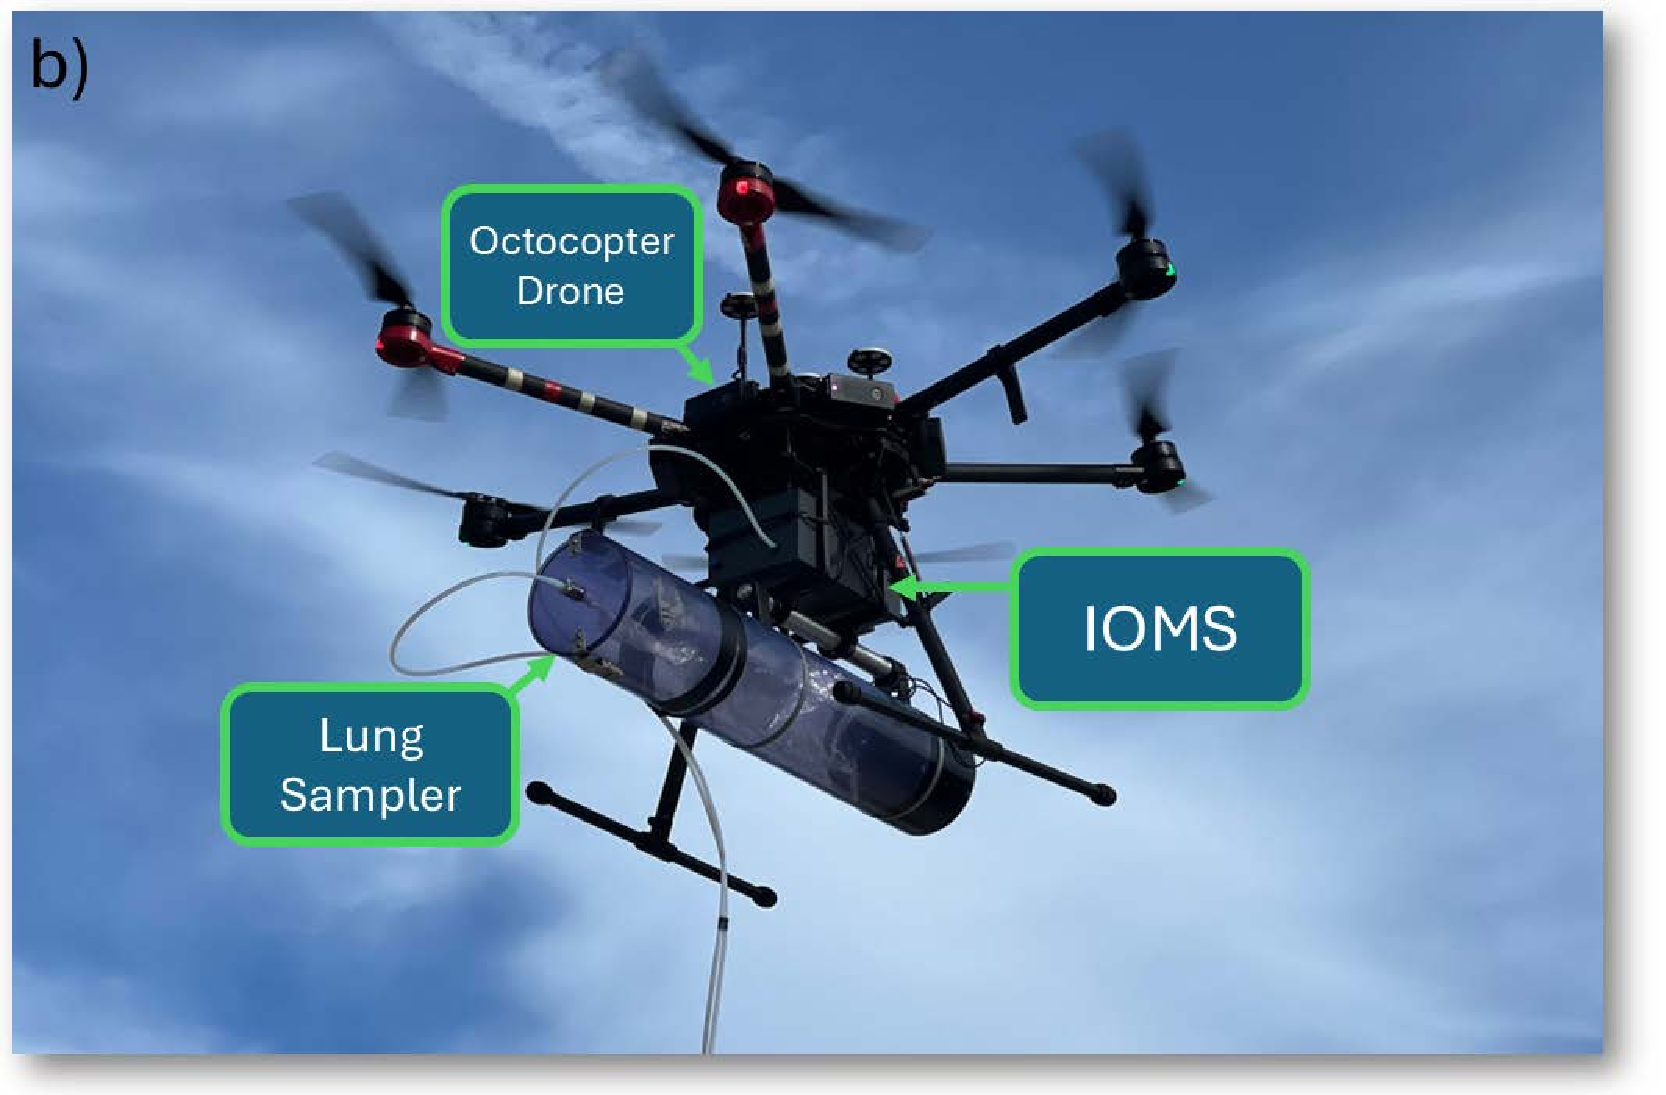
\includegraphics[width=\linewidth]{fig1b_2.pdf}
        \label{fig:ioms_b}
    \end{subfigure}
    
    \caption{IOMS onboarded in the flying drone. (a) Block Diagram of the onboarded IOMS. The drawing includes the communications modules, the lung sampler and the batteries. (b) Onboarded Hardware in the DJI octocopter. The figure shows the drone, the IOMS and the lung sampler.}
    \label{fig:ioms}
\end{figure}

%The IOMS consists of a Gas Chamber with 5 electrochemical sensors and 16 MOX sensors in a 96 cm3 volume, all listed in tables \ref{tab:echSensors} and \ref{tab:moxSensors}. All the electrochemical sensors were bought from Alphasense Inc. and they are interfaced with a microcontroller from Libellium via proprietary Analog Frontends. The MOX sensors belong to the TGS series from Figaro. As is described in Table 1, series of TGS2600, TGS2602, TGS2611 and TGS2620 are heated up by applying different voltages using PWM signals, which lead to different temperatures \cite{Fonollosa2013,Burgués2018}. The PWM signals are produced by an Arduino device and conditioned for power transfer by a custom-made electronic platform.


The Instrumental Odour Monitoring System (IOMS) features a gas chamber containing 5 electrochemical sensors and 16 MOX sensors within a 96 cm$^{3}$ volume, as detailed in Tables \ref{tab:echSensors} and \ref{tab:moxSensors}. The electrochemical sensors, sourced from Alphasense Inc., are connected to a Libellium microcontroller via proprietary analog frontends. The MOX sensors, part of the Figaro TGS series, include the models TGS2600, TGS2602, TGS2611, and TGS2620. These sensors are heated to various temperatures by applying different voltages through PWM signals, as described in Table 1 \cite{Fonollosa2013,Burgués2018}. The PWM signals are generated by an Arduino device and conditioned for power transfer using a custom-made electronic platform.

\begin{table}[ht]
    \centering
    \resizebox{\columnwidth}{!}{%
    \begin{tabular}{l l l l l}
        \toprule
        \textbf{} & \textbf{Technology} & \textbf{Range} & \textbf{Accuracy} & \textbf{Resp. time (T$_{90}$)} \\
        \midrule
        Flow rate & Ultrasonic & -33 to +33 L/min & ±3\% m.v. & $<$1 s \\
        CO$_2$ & NDIR & 0 to 5000 ppm & ±100 ppm & $<$60 s \\
        CO & Electrochemical & 0 to 100 ppm & ±0.5 ppm & $<$20 s \\
        H$_2$S & Electrochemical & 0 to 20 ppm & ±0.1 ppm & $<$20 s \\
        NH$_3$ & Electrochemical & 0 to 100 ppm & ±0.5 ppm & $<$90 s \\
        SO$_2$ & Electrochemical & 0 to 20 ppm & ±0.1 ppm & $<$45 s \\
        \bottomrule
    \end{tabular}
    } % Fin de resizebox
    \caption{Specifications of electrochemical, NDIR and Flow sensor}
    \label{tab:echSensors}
\end{table}

\begin{table}[ht]
    \centering
    \resizebox{\columnwidth}{!}{%
    \begin{tabular}{l l l l}
        \toprule
        \textbf{Sensor} & \textbf{Model} & \textbf{Target gases} & \textbf{Heater voltage (V)} \\
        \midrule
        M1,2,3,4  & TGS 2600 & H$_2$, CO, Ethanol & 1.6,3.2,4.0,4.9 \\
        M5,6,7,8  & TGS 2602 & H$_2$S, NH$_3$, Toluene & 1.6,3.2,4.0,4.9 \\
        M9,10,11,12  & TGS 2611 & CH$_4$, Hydrocarbons & 1.6,3.2,4.0,4.9 \\
        M13,14,15,16 & TGS 2620 & Alcohols, ketones & 1.6,3.2,4.0,4.2\\
        \bottomrule
    \end{tabular}
    } % Fin de resizebox
    \caption{Specifications of the MOX sensors included in the slave board}
    \label{tab:moxSensors}
\end{table}

%Fig.\ref{fig:ioms}(b) shows all the equipment onboarded in a DJI octocopter when flying. It includes the IOMS and the lung sampler used for collecting sample-bags filled with environmental air. Both, the IOMS and the lung sampler have a $10$~meters PTFE tube connected to their input. This distance is more than enough for avoiding down washing effect from the drone \cite{Yongjun2018,Zhu2021}. The tubes collect air from the same environment when the drone is flying over the plant.
Figure \ref{fig:ioms}(b) illustrates all the equipment mounted on a DJI octocopter during flight. This setup includes the IOMS and a lung sampler for collecting sample bags filled with environmental air. Both the IOMS and the lung sampler are connected to their inputs via 10-meter PTFE tubes. This length is sufficient to prevent the downwash effect from the drone \cite{Yongjun2018,Zhu2021}. The tubes ensure that air is collected from the same environment as the drone flies over the plant.

%The air is sucked with a Vacuum pump and the airflow is measured with a flow sensor also described in table \ref{tab:echSensors}. Every data produced by the sensors (electrochemical, MOX and flow sensor) is collected by the Libellium microcontroller and, among battery data, gps location data and other status data, is framed and sent via an Xbee module to a groundbased laptop. 
Air is drawn in using a vacuum pump, and the airflow is measured by a flow sensor, as detailed in Table \ref{tab:echSensors}. Data from electrochemical sensors, MOX sensors, and the flow sensor are collected by the Libellium microcontroller. This data, along with battery status, GPS location, and other system status information, is framed and transmitted via an Xbee module to a ground-based laptop.

%The laptop runs a custom-made software that collects the data sent by the IOMS via Xbee, record it and plots the results on the screen. The software also allows the user to command the IOMS to activate the lung sampler, making the readings from the sensors synchronized with the air filling the bug inside the lung sampler. Bags are usually collected at different locations in the WWTP and transported to a certified company which perform dynamic olfactometric analysis with the air inside the bags. Once the odour quantification is provided by the company, the data recorded from the sensors at each location and the odour quantification in $\nicefrac{OU_{E}}{m^{3}}$ are used to calibrate a odour prediction model.
%For more information about the IOMS consult previous work \cite{Burgues2020,Burgues2021}

The laptop runs custom-made software that collects data sent by the IOMS via Xbee, records it, and displays the results on the screen. The software also allows the user to command the IOMS to activate the lung sampler, synchronizing sensor readings with the air filling the bag inside the lung sampler. Bags are typically collected at various locations within the WWTP and transported to a certified company for dynamic olfactometric analysis. Once the odour quantification is provided by the company, the sensor data from each location and the odour quantification in $\nicefrac{OU_{E}}{m^{3}}$ are used to calibrate an odour prediction model. For more information about the IOMS, consult previous work \cite{Burgues2020,Burgues2021}.

\subsection{Measurement Campaign}
\label{ssec:measCamp}
Fig.\ref{fig:wwtp} shows the WWTP where the measurement campaign was performed. It is located in the south-west of Spain and presents a typical topology of a WWTP. 

\begin{figure}[ht!]
    \centering
    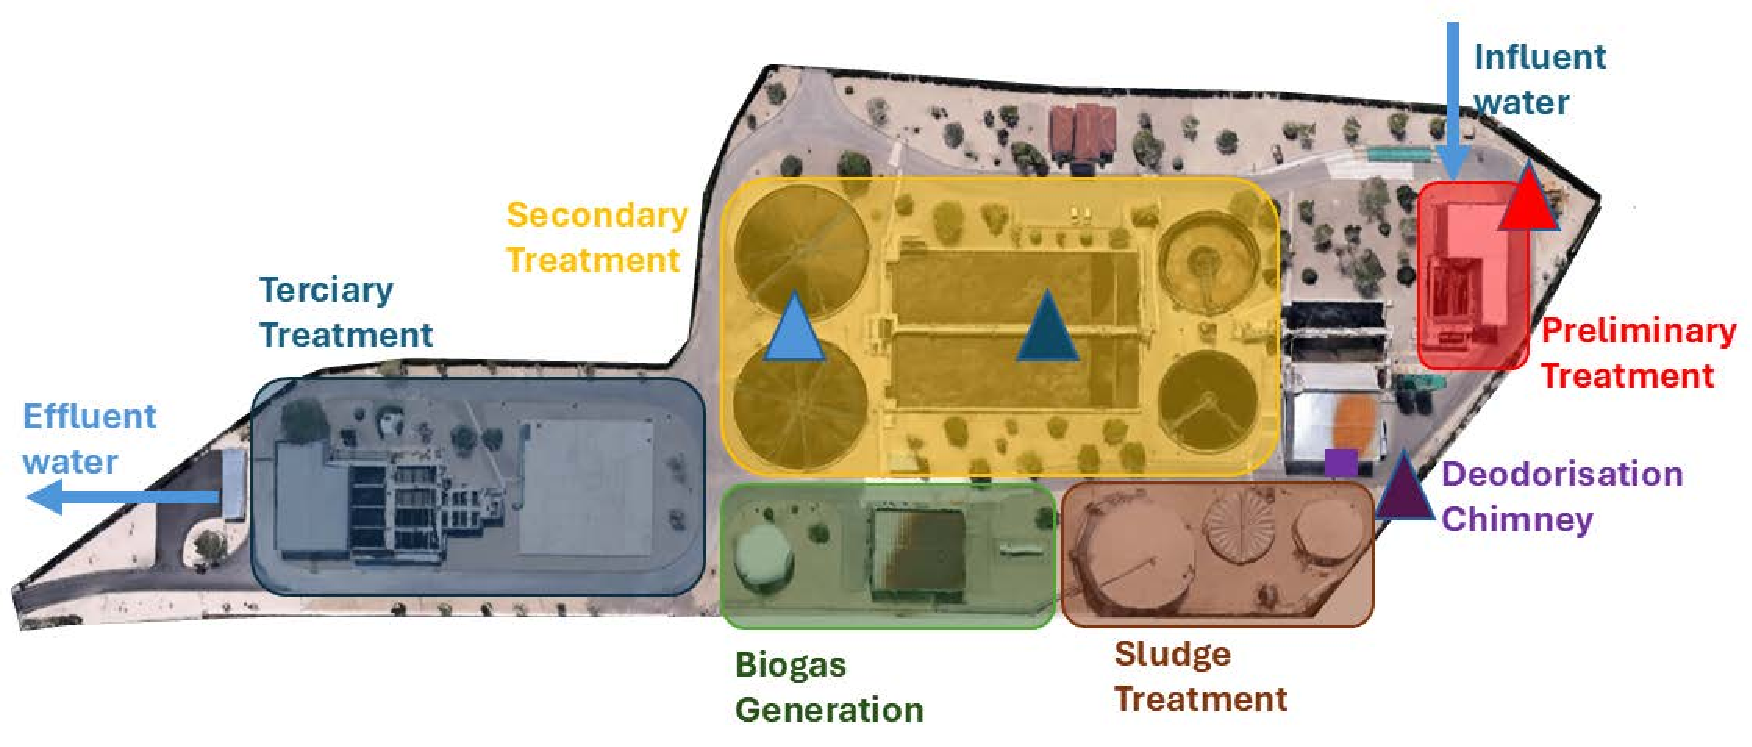
\includegraphics[width=1\linewidth]{fig2_2.pdf}
    \caption{Waste Water Treatment Plant where the measurement campaign was performed. \triangleup[cyan] Primary Settler, \triangleup[blue] Bioreactor, \triangleup[red] Preliminary Treatment Building, \triangleup[violet] Deodorisation Chimney.}
    \label{fig:wwtp}
\end{figure}

\begin{table}[ht]
    \centering
    \resizebox{\columnwidth}{!}{%
    \begin{tabular}{c c c c c c c c c c}
        \toprule
        \textbf{Day} & \textbf{Date} & \textbf{Settler}\triangleup[cyan] & \textbf{Bioreactor}\triangleup[blue] & \textbf{Pretreatment}\triangleup[red] & \textbf{Chimney}\triangleup[violet] & \textbf{Total (odour)} & \textbf{Blanks} & \textbf{Total} \\
        \midrule
        1 & 24/06/2020 & 3 & 3 & 2 & 2 & 10 & 7 & 17 \\
        2 & 25/06/2020 & 2 & 2 & 2 & 2 & 8 & 6 & 14 \\
        3 & 14/07/2020 & 3 & 3 & 3 & 3 & 12 & 11 & 23 \\
        4 & 15/07/2020 & 3 & 3 & 3 & 3 & 12 & 7 & 19 \\
        \midrule
        \textbf{Total} & & 11 & 11 & 10 & 10 & 42 & 31 & 73 \\
        \bottomrule
    \end{tabular}
    } % Fin de resizebox
    \caption{Number of samples collected in each source during the four measurement days}
    \label{tab:wwtpMeas}
\end{table}

%The major contribution on the odour level at each source is the combination of the gases emitted by the source itself \cite{Capelli2008}. Environmental factors (wind, temperature, humidity) have also influence in the odour level but under the same conditions, it is the source emission which determines the odour level when performing dynamic olfactometries \cite{Campos2016}. The Primary Settler (\triangleup[cyan] in Fig.\ref{fig:wwtp}) is typically a source of xxxx and the Bioreactor and the Preliminary Treatment Building (\triangleup[blue] and \triangleup[red] in Fig.\ref{fig:wwtp}) are tipically sources of xxxx. Finally, the Deodorisation Chimney (\triangleup[violet] in Fig.\ref{fig:wwtp}) is usually a source of xxxx.     
The primary factor influencing odour levels at each source is the combination of gases emitted by the source itself \cite{Capelli2008}. While environmental factors such as wind, temperature, and humidity also affect odour levels, the source emissions are the main determinant under consistent conditions when performing dynamic olfactometries \cite{Campos2016}. The Primary Settler (\triangleup[cyan] in Fig.\ref{fig:wwtp}) typically emits gases such as hydrogen sulphide (H$_2$S) and methane (CH$_4$) \cite{EPA2004}. The Bioreactor and the Preliminary Treatment Building (\triangleup[blue] and \triangleup[red] in Fig.\ref{fig:wwtp}) are common sources of carbon dioxide (CO$_2$), methane (CH$_4$), and nitrous oxide (N$_2$O) \cite{Campos2016}. Finally, the Deodorisation Chimney (\triangleup[violet] in Fig.\ref{fig:wwtp}) usually emits volatile organic compounds (VOCs) and hydrogen sulphide (H$_2$S) \cite{Casaca2022}.

%The campaign consisted in $4$ days of measurements with the drone flying over the $4$ sources. Table \ref{tab:wwtpMeas} summarizes the measurements. Each day at least two bags were collected at each source, each of them at different heights. Also, locations where the odour level was low (called blanks in Table \ref{tab:wwtpMeas}) were sampled. Fig.\ref{fig:rawData} shows the readings from the different sensors obtained in the first day of the measurement campaign.
%For more information about the IOMS consult previous work \cite{Burgues2020,Burgues2021}
The campaign spanned four days, during which the drone conducted measurements over four sources. Table \ref{tab:wwtpMeas} provides a summary of these measurements. Each day, at least two sample bags were collected from each source at different heights. Additionally, locations with low odour levels (referred to as blanks in Table \ref{tab:wwtpMeas}) were also sampled. Figure \ref{fig:rawData} displays the sensor readings obtained on the first day of the measurement campaign. For more information about the IOMS, please refer to previous work \cite{Burgues2020,Burgues2021}.

\begin{figure}[ht!]
    \centering
    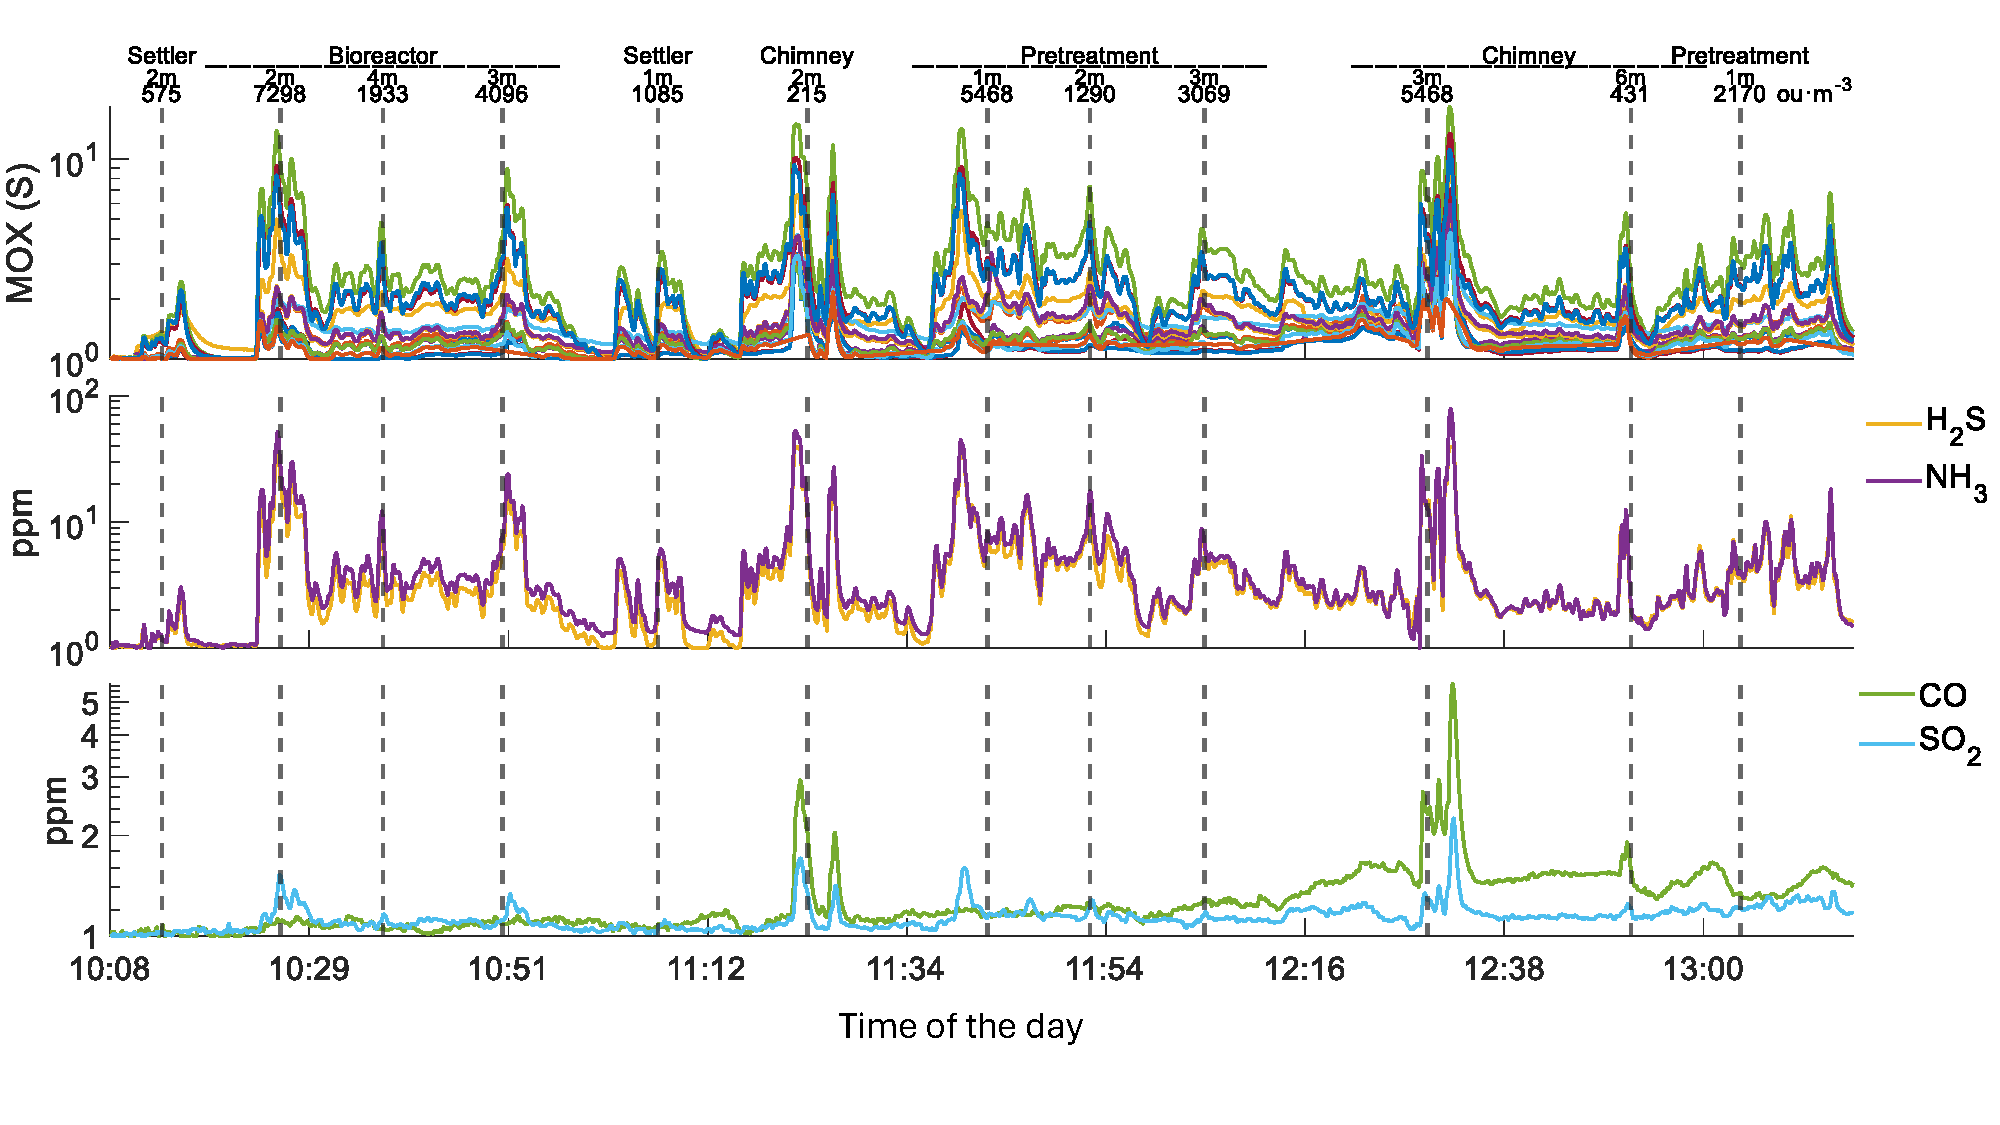
\includegraphics[width=1\linewidth]{fig3_2.pdf}
    \caption{Sensor readings in the first day of campaign. The figure includes the response of the $16$ MOX sensors, the H$_{2}$S and the NH$_{3}$ sensors, the CO and the SO$_{2}$ sensors, and the CO$_{2}$ sensor. The vertical pink bars indicate the moment when the lung sampler was on.}
    \label{fig:rawData}
\end{figure}


\subsection{General Workflow}
\label{ssec:genWorkflow}

%The data analysis performed to produce an odour level prediction model is depicted in Fig.\ref{fig:genWorkflow}(a). In this figure, a general overview of the training and validation process is presented accordingly with previous publications \cite{Burgues2020,Burgues2021_Ar,Burgues2021}. 
The data analysis process for developing an odour level prediction model is illustrated in Fig.\ref{fig:genWorkflow}(a). This figure provides a general overview of the training and validation process, consistent with previous publications \cite{Burgues2020,Burgues2021_Ar,Burgues2021}.

\begin{figure}[ht]
    \centering
    % Primera subfigura
    \begin{subfigure}[b]{\columnwidth}
        \centering
        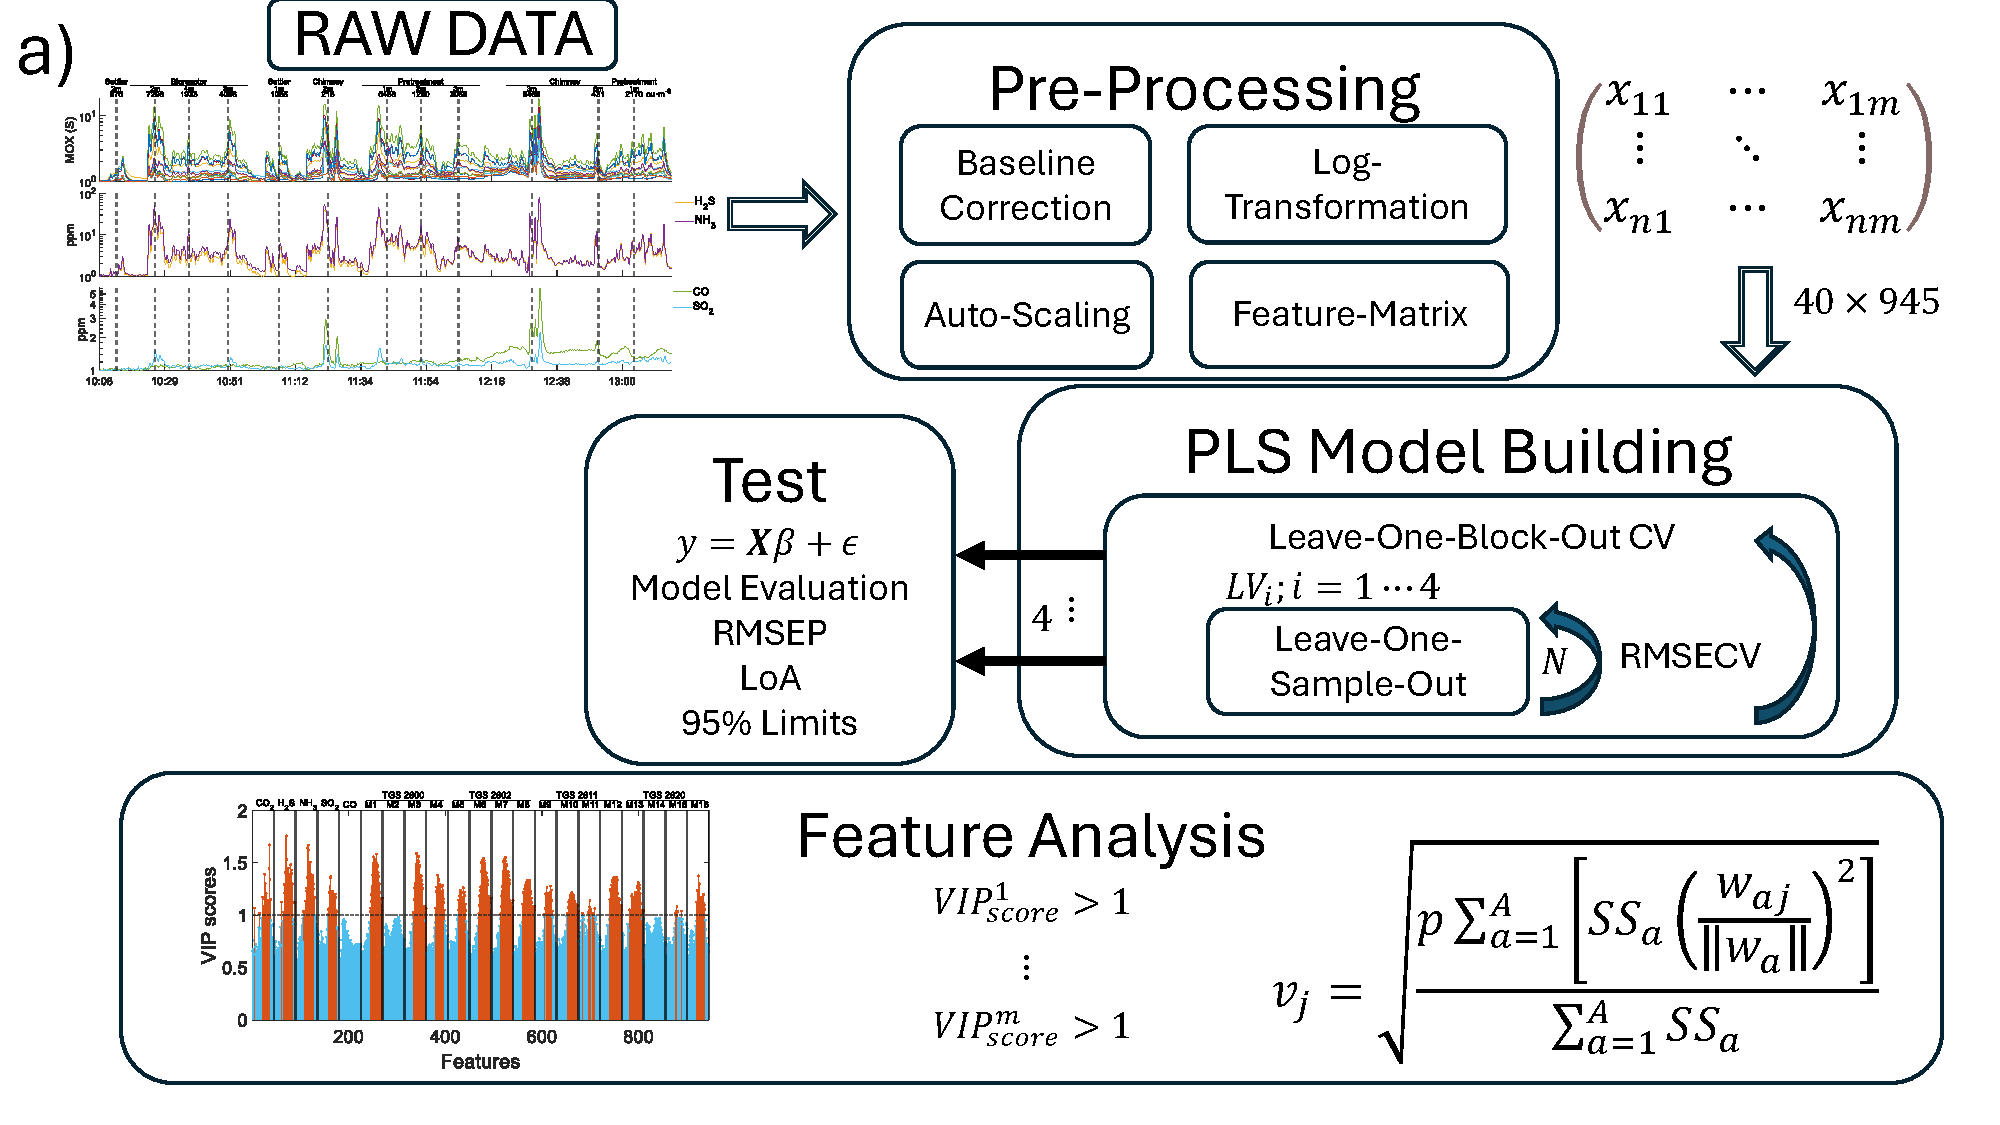
\includegraphics[width=\linewidth]{fig4a_3.pdf}
        \label{figbgenWorkflow_a}
    \end{subfigure}
    
    % Segunda subfigura (la misma imagen)
    \begin{subfigure}[b]{\columnwidth}
        \centering
        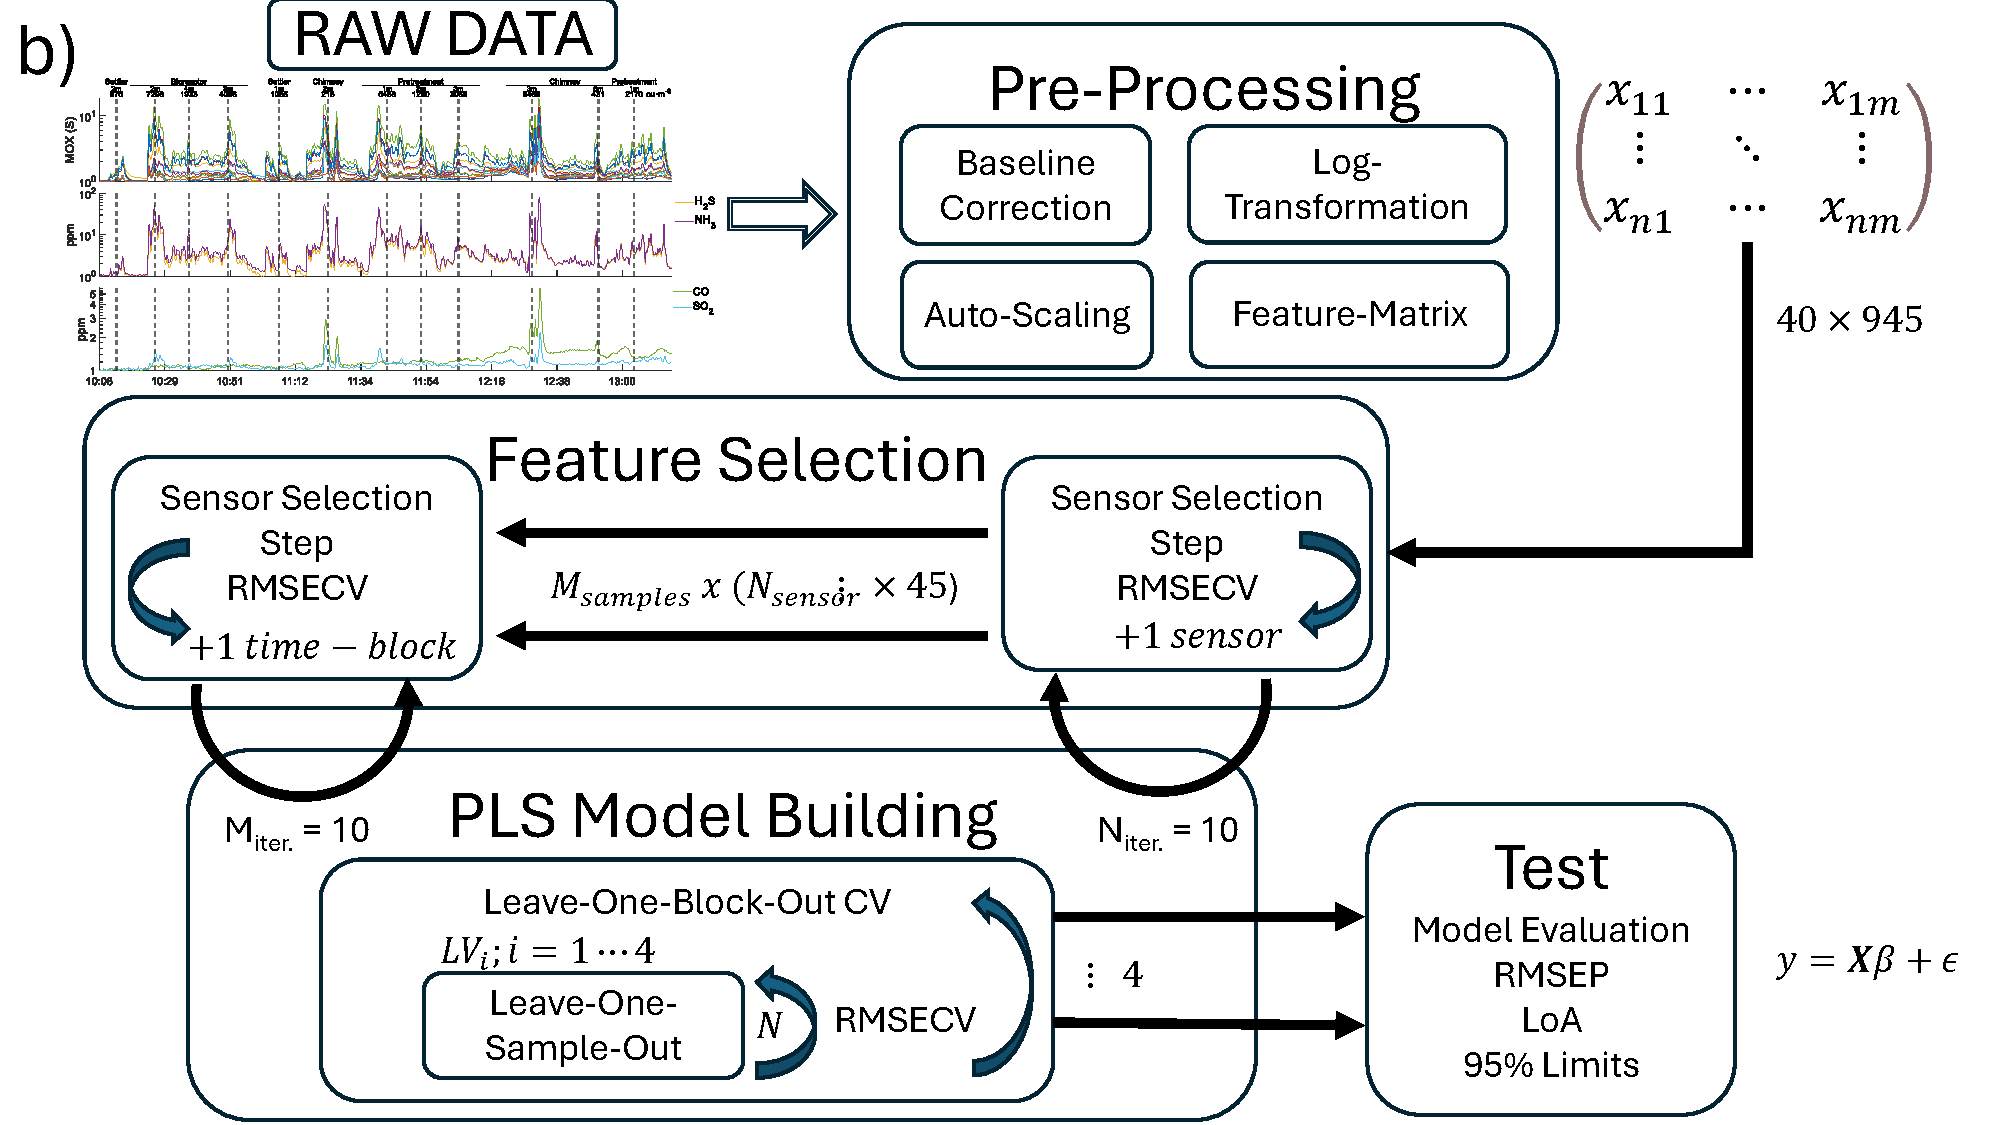
\includegraphics[width=\linewidth]{fig4b_3.pdf}
        \label{fig:genWorkflow_b}
    \end{subfigure}
    
    \caption{Data analysis Workflow. (a) General Workflow with Feature Selection based on VIP calculation and discrimination. (b) Modified Workflow with NiPLS as Feature Selection methodology.}
    \label{fig:genWorkflow}
\end{figure}

Firstly, the sensor readings are pre-processed using different techniques for MOX sensors and Electrochemical sensors. After a baseline correction for each sensor, a log-transformation was applied at every data sequence recorded with the IOMS. The Feature matrix was organized forming a total matrix of $nxm$ rows and columns, where each row corresponds to a sampling bag collected with the lung sampler and each column to a single value of the sensor readings. 

%The vertical lines at Fig.\ref{fig:rawData} mark when the lung sampler is activated. Around this marks, 5 minutes are considered as relevant for the analysis. The rest of the time series is removed from the features. In total the feature matrix has dimensions of $73x945$ including blancs for pre-processing purposes (73 samples by 21 sensors multiplied by 45 $\nicefrac{samples}{sensor}$). After using the blancs and leaving not-useful samples out of the matrix, the final feature matrix consists in $40x945$ matrix where each sensor has 45 features at each sample.
The vertical lines in Fig.\ref{fig:rawData} indicate when the lung sampler is activated. Around these marks, 5 minutes are considered relevant for the analysis, and the rest of the time series is excluded from the features. The initial feature matrix has dimensions of $73x945$, including blanks for pre-processing purposes (73 samples by 21 sensors multiplied by 45 samples per sensor). After removing the blanks and excluding non-useful samples, the final feature matrix consists of $40x945$, where each sensor has 45 features per sample.

%Once the feature matrix is built, a Partial Least Squares model is trained and tested as explained in \cite{Wold2001}. A double leave-one-block-out cross-validation (CV) scheme is performed for model building. This scheme takes three days for model training and leaves out one day for validation producing $4$ different models from the one with best performance is chosen. 


%Once the feature matrix is constructed, a Partial Least Squares (PLS) model is trained and tested as described in \cite{Wold2001}. A double leave-one-block-out cross-validation (CV) scheme is employed for model building. This approach uses data from three days for model training and reserves one day for validation, resulting in four different models. The model with the best performance is then selected. The Variable Importance Projection (VIP) method is in order to get information about the most relevant features in training. The VIPs of each sensor are averaged per day at every feature (45 per sample for each sensor), leading to an averaged VIP score distribution depicted in Fig. \ref{fig:rawDetail}~(b).
Once the feature matrix is constructed, a Partial Least Squares (PLS) model is trained and tested as described in \cite{Wold2001}. A double leave-one-block-out cross-validation (CV) scheme is employed for model building. This approach uses data from three days for model training and reserves one day for validation, resulting in four different models. The model with the best performance is then selected. 

In order to avoid complexity grow uncontrolled at each of the proposed models, within each calibration set the “leave one sample out” (LOO) scheme is used. N PLS models are built with different Latent Variables (LVs) leaving a sample for test out of the building process. The number of LVs is therefore optimized by evaluating the Root Mean Square Error in Cross Validation (RMSECV). Finally, the models are refit using the calibration samples used during training and used to produce prediction plots on blind samples. The bias of the prediction and 95\% limits of agreement (LoA) are computed using the Bland-Altman methodology \cite{Taffe2021}. 

Whenever the model is ready for predictions, the Variable Importance in Projection (VIP) method is used to identify the most relevant features during training. The VIP scores of each sensor are averaged per day for each feature (45 per sample for each sensor), leading to an averaged VIP score distribution depicted in Fig. \ref{fig:rawDetail}~(b).

\subsection{Nested Sequential Forward Selector using iPLS for Odour Quantification}
\label{ssec:NiPLS}
%The presented workflow is optimal for dataset with low number of samples. In the performed measurement campaign this number reduces to $73$ where almost half of the samples correspond to blank samples used for signal correction. Its strength is based in the Cross Validation technique that performs Leave-one Block-Out and Leave-one Sample-Out nested to get optimized models. However, the feature selection is performed using a more general procedure and it does not take into account the peculiarities of the acquired dataset. 
The presented workflow is optimal for datasets with a low number of samples. In the performed measurement campaign, this number reduces to 73, with almost half of the samples corresponding to blank samples used for signal correction. Its strength lies in the cross-validation technique, which performs nested leave-one-block-out and leave-one-sample-out procedures to optimize models. However, no feature selection was performed in the workflow, leaving the information from the extracted features unexploited. 

Figure \ref{fig:genWorkflow}(b) shows the modified data analysis workflow proposed to optimize the model training presented in Section \ref{ssec:genWorkflow} and depicted in Fig. \ref{fig:genWorkflow}(a). The proposed methodology is very similar to the one applied for cross-validation (CV) in the general workflow but incorporates a two-step feature selection process. This feature selection stage is based on the Nested Sequential Forward Algorithm. 

 In the first step of the feature selection stage, a PLS model is built using the general workflow but including only one sensor of the sequence of 945 features of each sample. The RMSECV is calculated and then another PLS model is built adding a different sensor to the previous one. The process is iterated $10$ times looking for a minimum in the RMSCEV. As depicted in Fig.\ref{fig:NiPLS}(a), at each iteration, a table informing the configuration of the sensors is created. The table provides information about which sensors are included in the feature matrix (\squarecolor[yellow]) and which are not (\squarecolor[teal]). 

 In the second step of the feature selection stage, a time-slot of each sensor around the activation of the lung sampler (the $5$ minutes window corresponding to the vertical bar in Fig.\ref{fig:rawData}) is divided in $15$ blocks, which corresponds to time-blocks of 20 seconds. With this partition, a similar procedure than the one described in the Sensor step is performed. Time-blocks are added to the model building process and the RMSECV is observed. After $10$ iterations a minimum appears to be clear for a selection of time-blocks. 


\section{Results and Discussion}
\label{sec:results}

\subsection{Gas Concentration Measurements}
\label{ssec:gasMeas}

%Fig.~\ref{fig:rawData} shows an example of data collected by the IOMS during a day of campaign. Data collected from the different sensors is pre-processed using the different blanc samples and baseline level is corrected with the lowest value of the day recorded for each sensor. After this adjustment, the 5 minutes time-slot around the sampling bag filling (\squarecolor[pink] rectangle in Fig.~\ref{fig:rawData}, which correspond to 45 samples) is placed in the feature matrix as explained in Fig.~\ref{fig:genWorkflow}. The final look of the feture matix after being pre-precossed according to the general workflow is depicted in Fig.~\ref{fig:preprocData}.   
Figure \ref{fig:rawData} shows an example of data collected by the IOMS during a day of the campaign. Data from the different sensors is pre-processed using the blank samples, and the baseline level is corrected with the lowest value recorded for each sensor that day. After this adjustment, the 5-minute time slot around the sampling bag filling (\squarecolor[pink] rectangle in Fig.\ref{fig:rawData}, corresponding to 45 samples) is included in the feature matrix as explained in Fig.\ref{fig:genWorkflow}. The final appearance of the feature matrix after pre-processing according to the general workflow is depicted in Fig.~\ref{fig:preprocData}.

\begin{figure}[ht!]
    \centering
    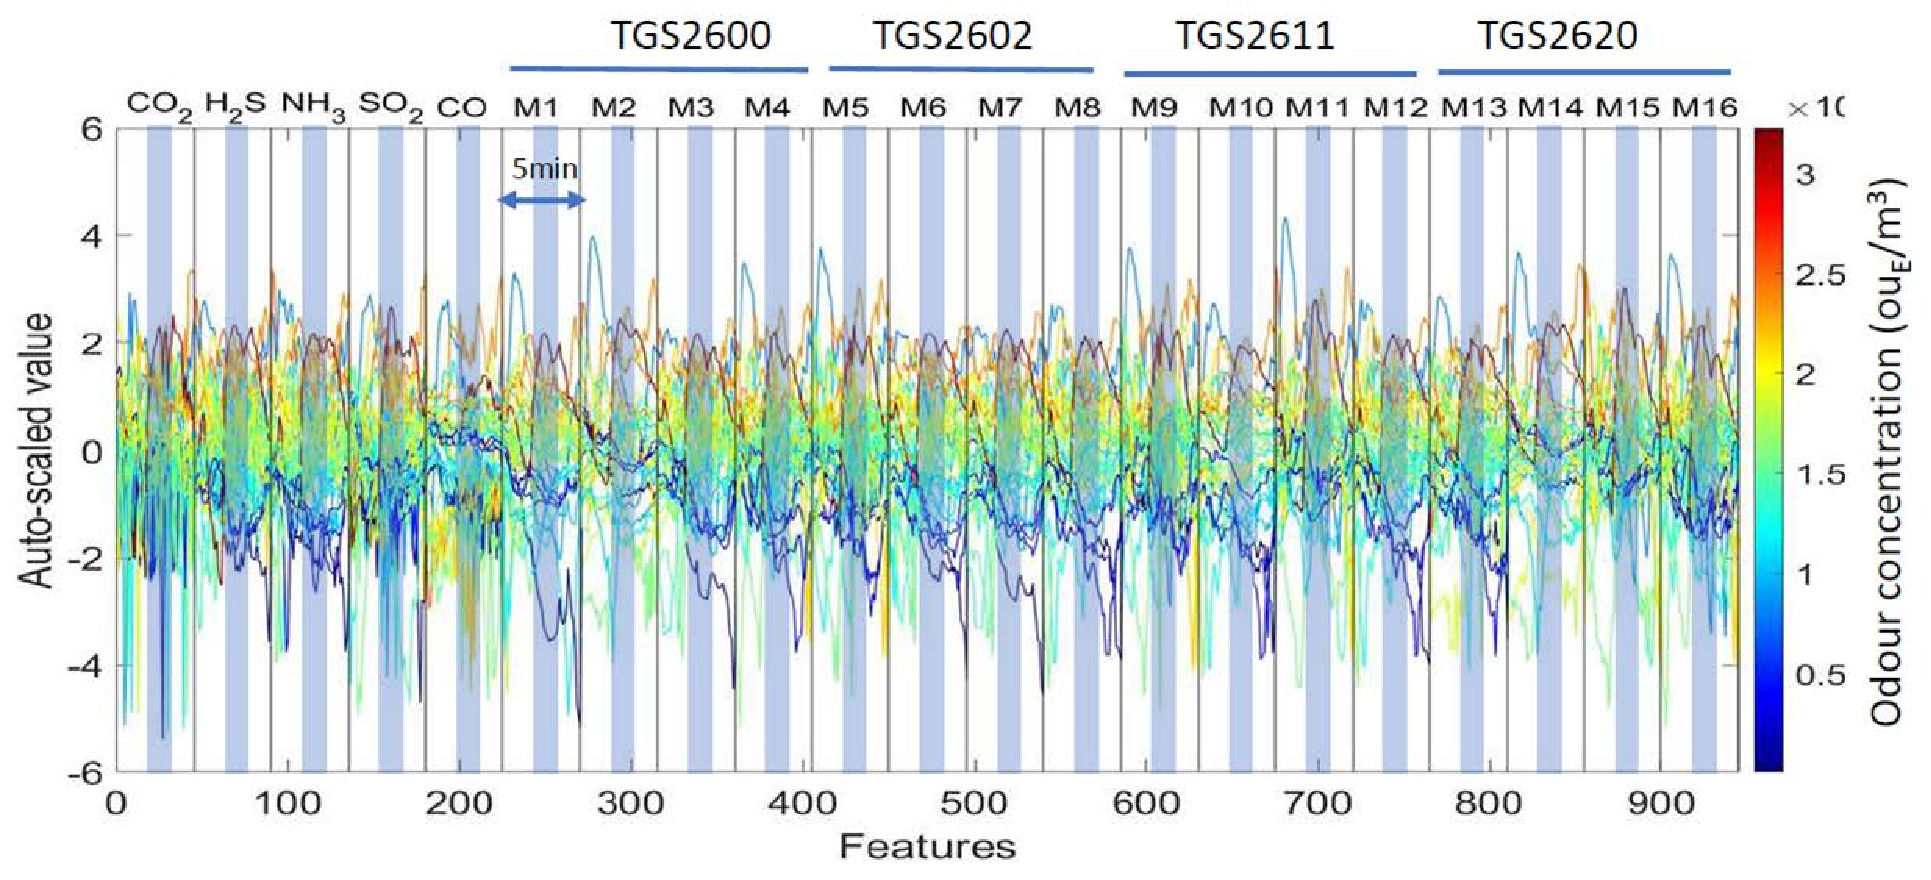
\includegraphics[width=1\linewidth]{Fig7.pdf}
    \caption{Preprocessed data of the different sources for every day of the measurement campaign. The 5 minutes of valid data have been marked in the plot.}
    \label{fig:preprocData}
\end{figure}

%A more detailed analysis is presented in Fig.~\ref{fig:rawDetail}. In this figure, the data from the H$_{2}$S and NH$_{3}$ sensors is depicted with the 5 minute time-slot marked with a pink rectangle (\squarecolor[pink]). This time-slot corresponds to the data included in the feature matrix for each sensor (see Fig.~\ref{fig:rawDetail}~(a)). 
A more detailed analysis is presented in Fig.\ref{fig:rawDetail}. This figure shows the data from the H$_{2}$S and NH$_{3}$ sensors, with the 5-minute time slot marked by a pink rectangle (\squarecolor[pink]). This time slot corresponds to the data included in the feature matrix for each sensor (see Fig.\ref{fig:rawDetail}~(a)).

\begin{figure}[ht!]
    \centering
    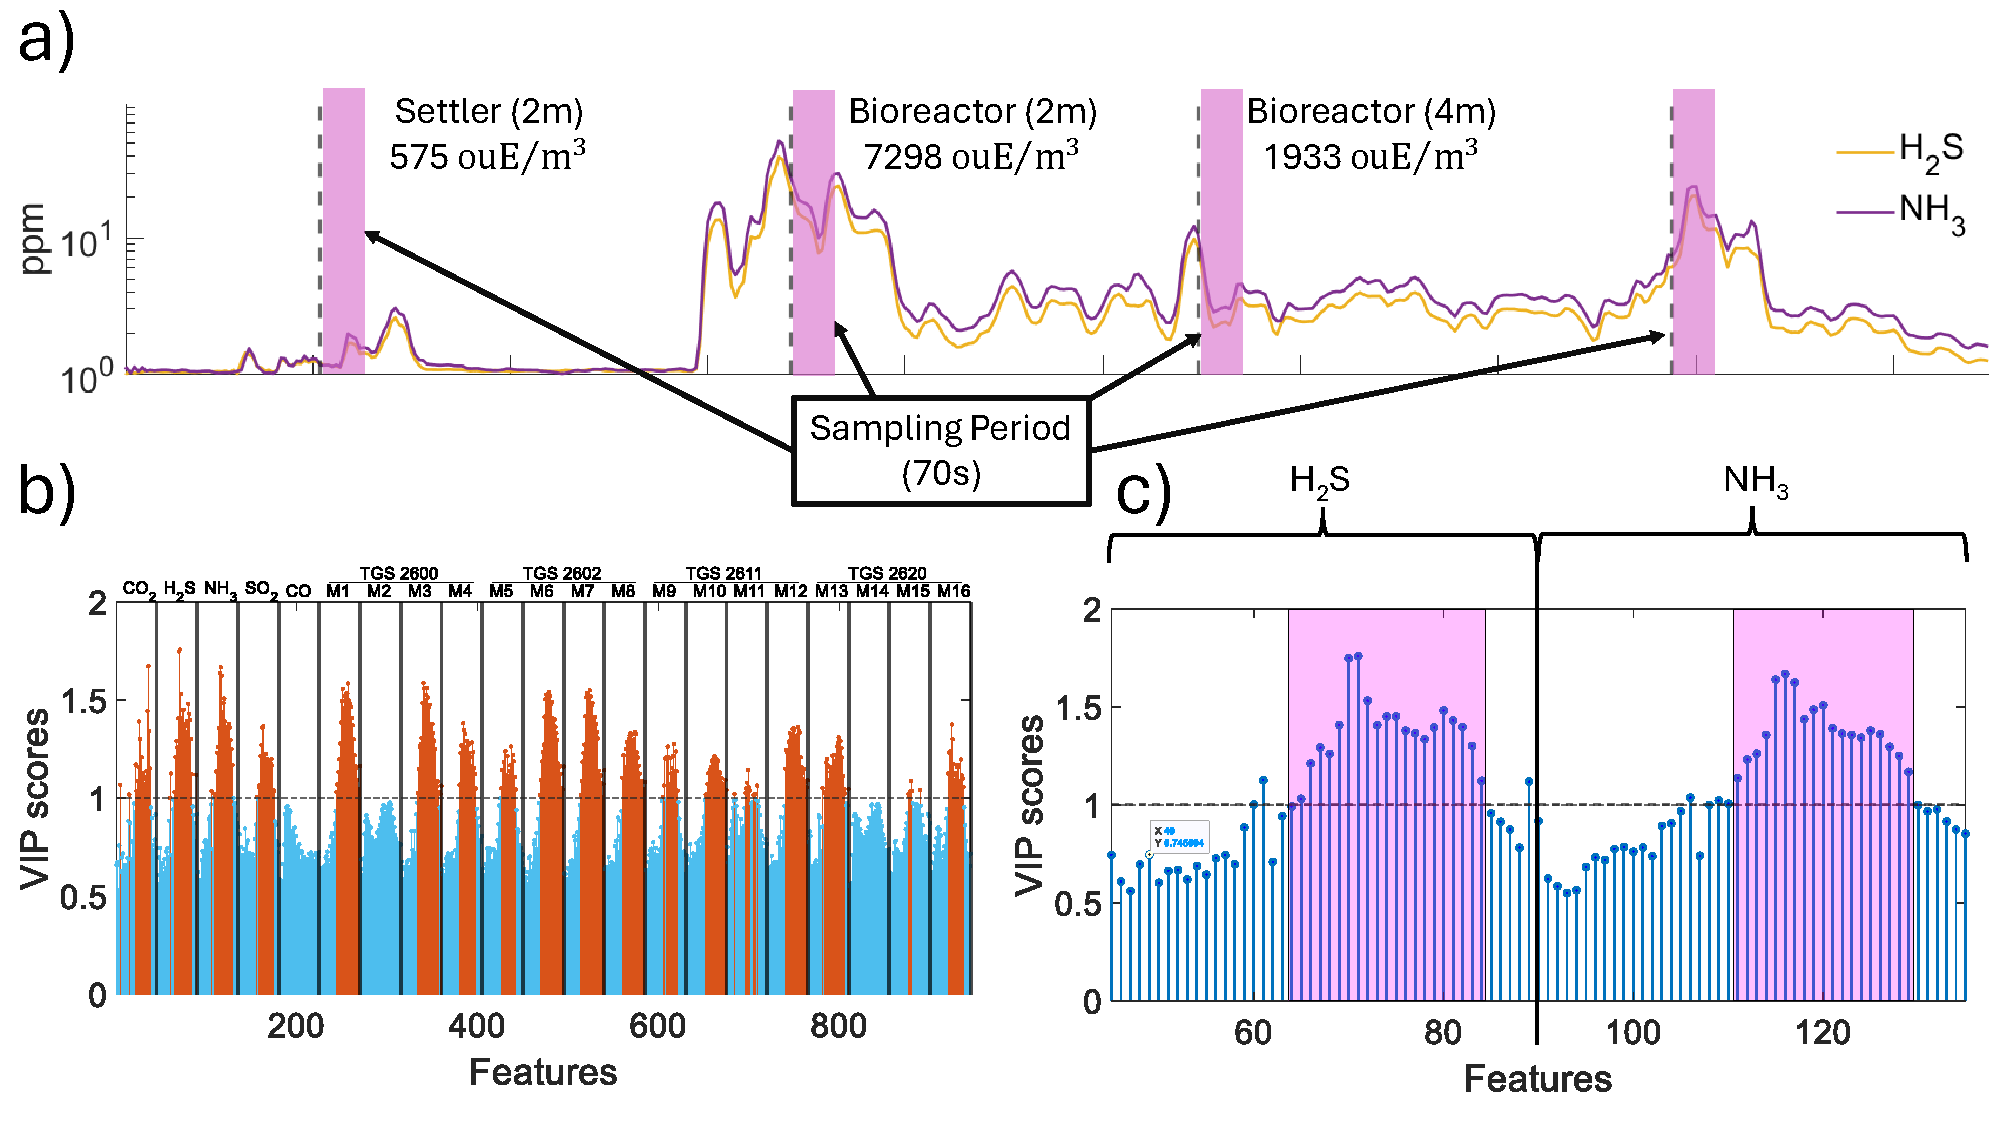
\includegraphics[width=1\linewidth]{fig6.pdf}
    \caption{Detail of the signal acquired from two of the most significant sensors (H$_{2}$S and NH$_{3}$) when the drone is flying over several sources and VIP scores. (a) Detail of the signal acquired and sampling period (\squarecolor[pink]). (b) Distribution of the VIP scores of every sensor when averaged over the four days of campaign at every time-slot. (c) Detail of the averaged VIP scores for H$_{2}$S and NH$_{3}$. The sampling period is also marked (\squarecolor[pink]).}
    \label{fig:rawDetail}
\end{figure}

%Fig.~\ref{fig:rawDetail}~(b) shows the VIP for each sensor averaged at each day computed as explained in Section \ref{ssec:genWorkflow}. The VIP analysis shows that inside the 5 minute-slot considered for each sensor, the most relevant features are commonly placed at the end of the sampling bag filling process. In particular, there are 21 samples which produce VIPs~$>1$. Also it is observed that the higher values for the VIP scores belong to the H$_{2}$S and NH$_{3}$ electrochemical sensors and some of the MOX sensors. Therefore, it should be possible to reduce the features used to train the prediction PLSR model by selecting the relevant sensors and the features of each relevant sensor in the 5 minute time-slot. 
Figure \ref{fig:rawDetail}~(b) shows the VIP for each sensor averaged per day, computed as explained in Section \ref{ssec:genWorkflow}. The VIP analysis indicates that within the 5-minute time slot considered for each sensor, the most relevant features are typically located at the end of the sampling bag filling process. Specifically, there are 21 samples with VIPs greater than 1. Additionally, the highest VIP scores are observed for the H$_{2}$S and NH$_{3}$ electrochemical sensors, as well as some of the MOX sensors. Therefore, it should be possible to reduce the features used to train the prediction PLSR model by selecting the relevant sensors and the features of each relevant sensor within the 5-minute time slot.

\subsection{General Workflow Performance}
\label{ssec:workflowPerf}
In orther to compare the performance of the NiPLS workflow with workflows presented in the literature \cite{Burgues2021,Burgues2021_Ar} the performance of the workflow depicted in Fig.~\ref{fig:genWorkflow}~(a) is presented in Fig.~\ref{fig:worflowPerf}.

\begin{figure}[ht!]
    \centering
    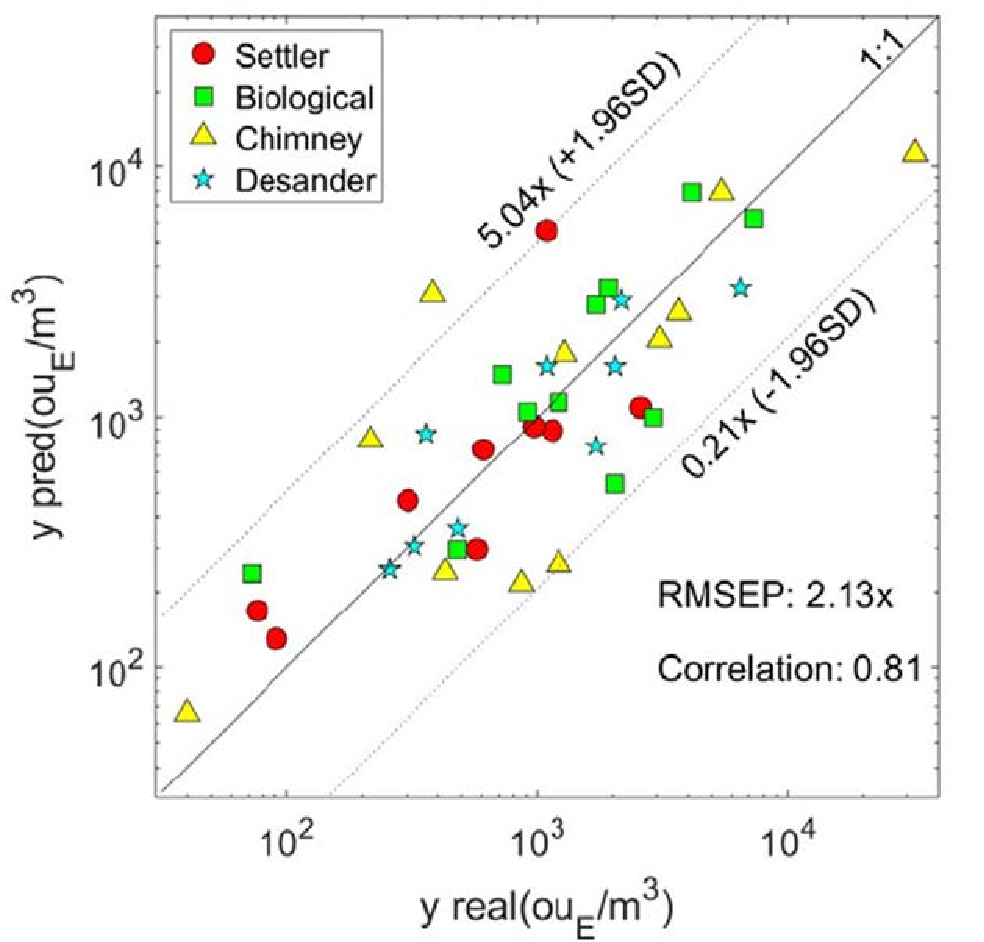
\includegraphics[width=1\linewidth]{fig7_3.pdf}
    \caption{Performance of the general workflow presented in section \ref{ssec:genWorkflow}. The number of useful samples have been reduced to 40 plus blanks.  Prediction plot for the best PLS model built with LoA limits at 95\% CI of $[0.2x-5.0x]$ and correlation coefficient of 0.81.}
    \label{fig:worflowPerf}
\end{figure}

%In this case, when $40$ samples are considered (from the $73$ acquired and after removing blancs) the best PLRS model presente $2$ Latent Variables. This model obtains an RMSEP of $2.13$x for 4 sources considered at different heights, the Settler (\triangleup[cyan]), the Bioreactor (\triangleup[blue]), the Chimney (\triangleup[violet]) and the Pretreatment Building (\triangleup[red]). In this case the calculated LoA at $95$\% CI lies in the $0.2$x to $5$x range of the prediction.
In this case, when $40$ samples are considered (from the $73$ acquired, after removing blanks), the best PLSR model presents 2 latent variables. This model achieves an RMSEP of $2.13$x for the $4$ sources considered at different heights: the Settler (\triangleup[cyan]), the Bioreactor (\triangleup[blue]), the Chimney (\triangleup[violet]), and the Pretreatment Building (\triangleup[red]). The calculated LoA at $95$\% CI ranges from $0.2$x to $5$x of the prediction.

\subsection{NiPLS Performance}
\label{ssec:NiPLSPerform}

With the NiPLS presented in Fig.~\ref{fig:genWorkflow}~(b) the results of the novel feature selection algorithm are presented. When the iPLS achieves the sixth and fifth iteration, the RMSECV goes down in both steps of the selection process (sensor step and time-slot step). 
\begin{figure}[ht!]
    \centering
    % Primera subfigura
    \begin{subfigure}[b]{\columnwidth}
        \centering
        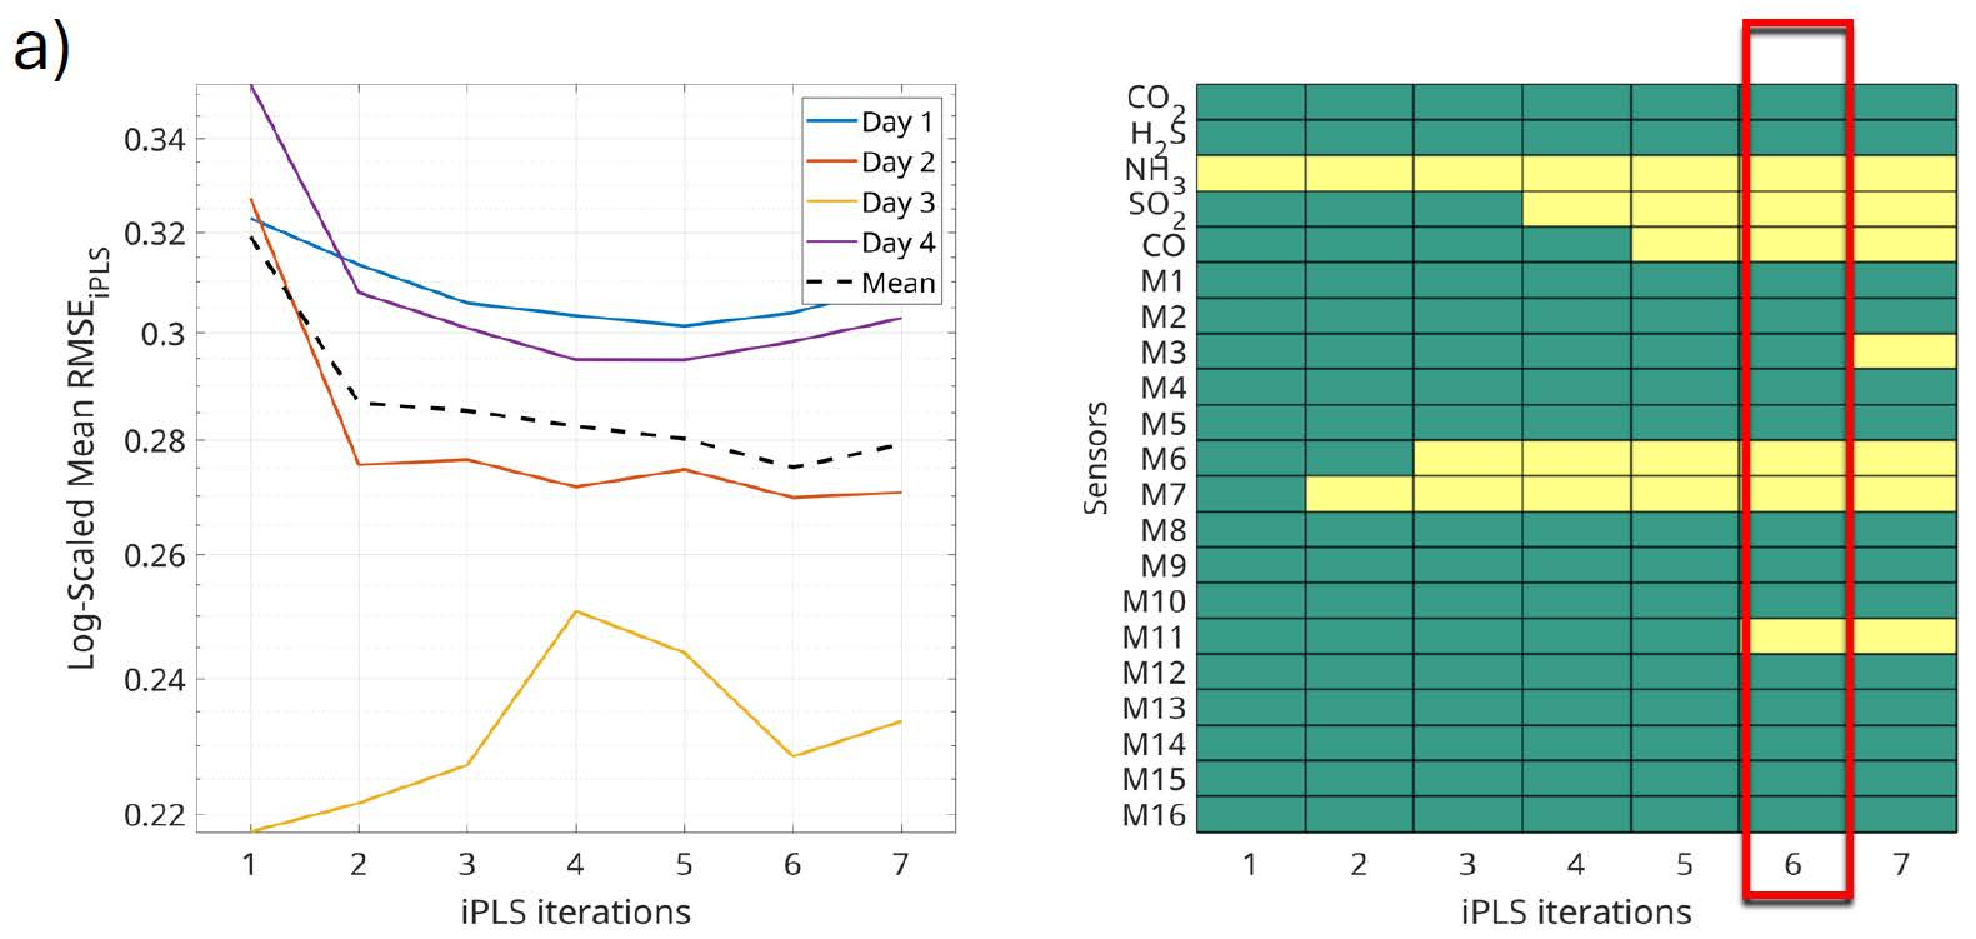
\includegraphics[width=\linewidth]{fig8a_3.pdf}
        \label{fig:NiPLS_a}
    \end{subfigure}
    
    % Segunda subfigura (la misma imagen)
    \begin{subfigure}[b]{\columnwidth}
        \centering
        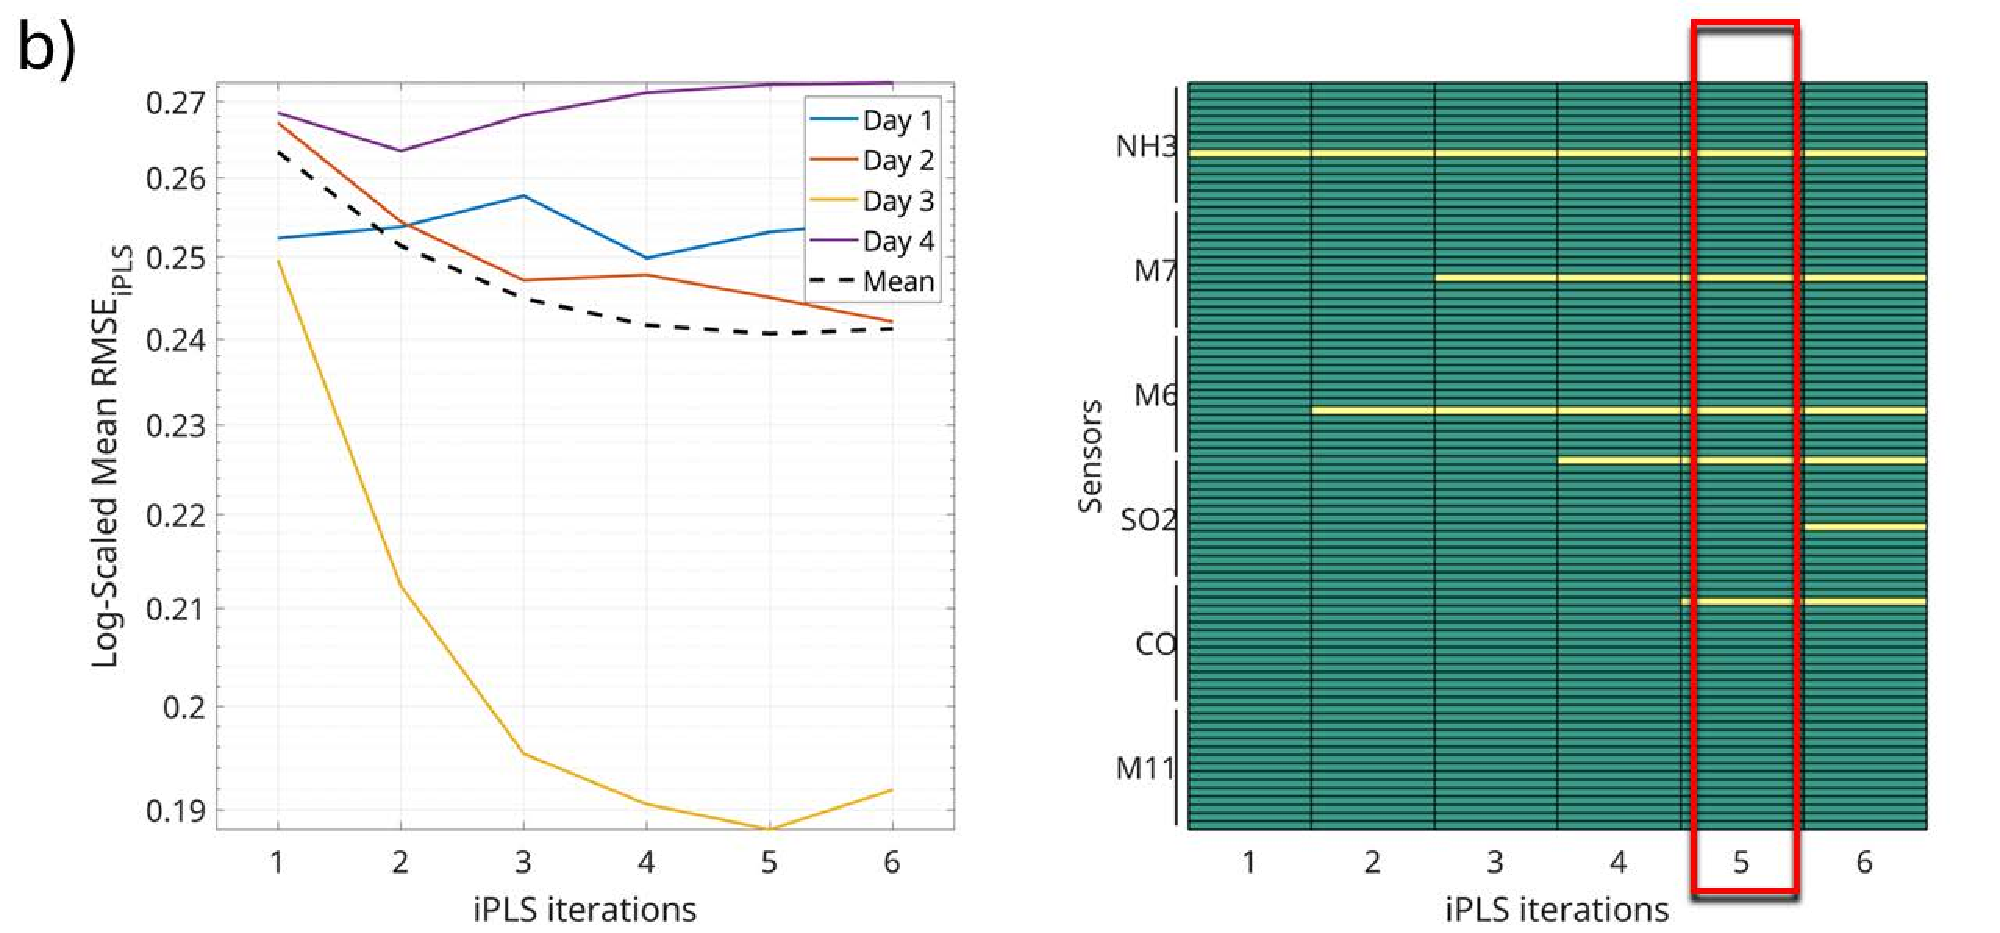
\includegraphics[width=\linewidth]{fig8b_2.pdf}
        \label{fig:NiPLS_b}
    \end{subfigure}
    
    \caption{Nested Sequential Forward Selector. The graphs show the evolution of the RMSECV for each day (and mean) during the block selection process. \squarecolor[yellow] interval included in the feature matrix, \squarecolor[teal] interval not included in the feature matrix (a) In the Sensor Step three electrochemical sensors (NH$_{3}$, SO$_{2}$ and CO) and three MOX sensors (M6, M7 TGS2602 and M11 TGS2611) show the maximum improvement in RMSECV. (b) In Time-slot Step the mid time-slot (15 seconds) of the NH$_{3}$, CO, M6 and M7 sensors improve even further the RMSECV.}
    \label{fig:NiPLS}
\end{figure}

%%In the sensor step, six sensors are selected as most relevant. The NH$_{3}$, SO$_{2}$ and CO from the electrochemical sensors and the MOX sensors M6, M7 and M11. These MOX sensors belong to the second (TGS2602) and the third (TGS2611) group of MOX sensors (see Table~\ref{tab:moxSensors}) at $3.2$~V, $4.0$~V and $4.0$~V respectively. 
In the sensor selection step, six sensors are identified as the most relevant: the NH${3}$, SO${2}$, and CO electrochemical sensors, and the MOX sensors M6, M7, and M11. These MOX sensors belong to the second (TGS2602) and third (TGS2611) groups of MOX sensors (see Table~\ref{tab:moxSensors}), operating at 3.2 V, 4.0 V, and 4.0 V, respectively.

%In the time-slot step, $5$ time-slot of the preselected sensors are selected as the most relevant features of these sensors. However, in this case the, features from the M11 MOX sensor are left out. For the NH$_{3}$, M7 and M6 sensors, the selected features correspond to the central part of the $45$ features and for the SO$_{2}$ and CO electrochemical sensors, the initial features seam to be more relevant. 
In the time-slot selection step, five time slots of the preselected sensors are chosen as the most relevant features. However, the features from the M11 MOX sensor are excluded. For the NH$_{3}$, M7, and M6 sensors, the selected features correspond to the central part of the $45$ features, while for the SO$_{2}$ and CO electrochemical sensors, the initial features appear to be more relevant.

With this features, the resulted PLSR model shows the performance depicted in Fig.~\ref{fig:NiPLSperformance}

\begin{figure}[ht!]
    \centering
    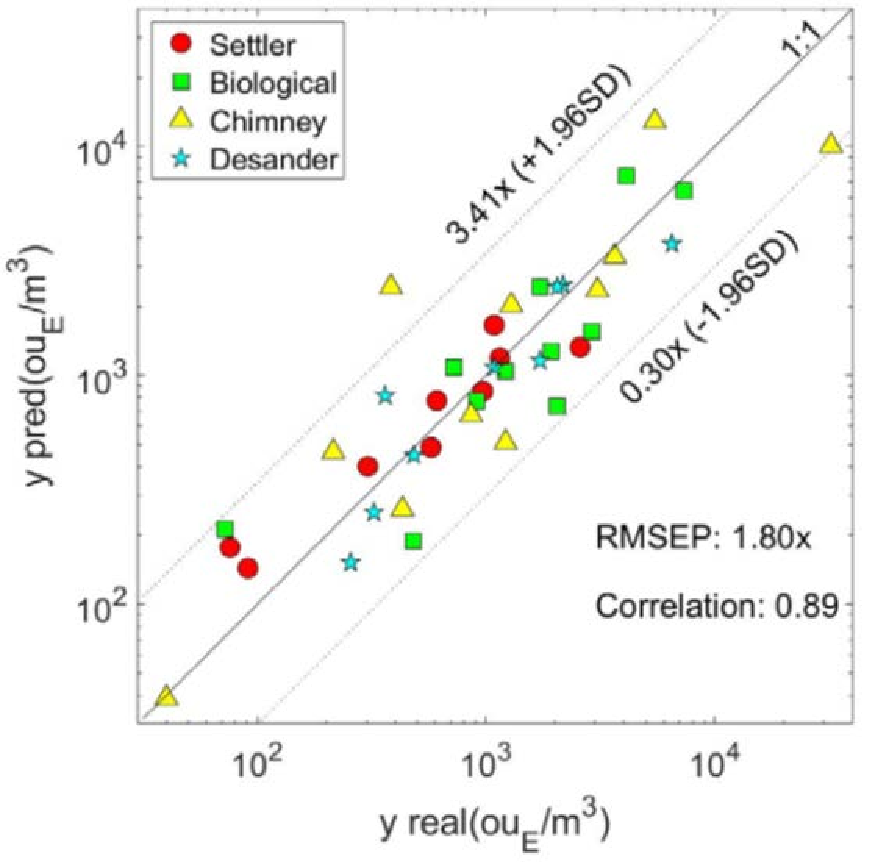
\includegraphics[width=1\linewidth]{fig9.pdf}
    \caption{Performance of the optimized model using NiPLS. The number of useful samples have been reduced to 40 plus blanks. The model shows LoA limits at 95\% CI of $[0.3x-3.4x]$ and a correlation coefficient of 0.89.}
    \label{fig:NiPLSperformance}
\end{figure}

%A reduction of the RMSEP is observed when the same set of samples used in Section~\ref{ssec:workflowPerf} is considered. The NiPLS model shows a RMSEP of 1.8x and the LoA at $95$\% CI lies in the $0.3$x to $3.4$x range, which is a considerable improvement when traditional feature selection is applied to the data set (see Fig.~\ref{fig:worflowPerf}).



A reduction in RMSEP is observed when the same set of samples used in Section~\ref{ssec:workflowPerf} is considered. The NiPLS model shows an RMSEP of $1.8$x, and the LoA at 95\% CI lies in the $0.3$x to $3.4$x range. This represents a considerable improvement compared to traditional workflow applied to the dataset (see Fig.~\ref{fig:workflowPerf}).

\section{Conclusions}
\label{sec:conclusions}
%In this contribution, a novel application of the Nested Sequential Forward Feature Selection algorithm is presented. Its combination with the Interval Partial Least Square Regression model, when modified accordingly for the special case of IOMSs studding odour concentrations in Waste Water Treatment Plants, proves to improve the performance of the model comparing with traditional approaches. In particular, for the measurement campaign performed in a WWTP in Spain, the novel workflow shows an improment on the RMSEP of 0.2 point and a reduction of the Limit of Agreement at $95$\% CI from $5$x to $3.4$x.

%These result enhances the performance of IOMS on-boarded in drones evaluating odour emission and allows to used it as a complementary odour analysis tool to the dynamic olfactometry in WWTPs.  

%Furthermore, the novel workflow shows relevant information when considering improvement on the IOMS. The information of the relevant sensors might be used to reduce the size and the data load transferred from the IOMS to the ground PC.
This contribution demonstrates how obtaining information on the importance of sensors and features enables the implementation of an algorithm to automatically select the most relevant information, resulting in improved model performance. By combining this approach with the Interval Partial Least Squares Regression model, specifically tailored for IOMSs studying odour concentrations in Wastewater Treatment Plants (WWTPs), significant enhancements are achieved compared to traditional methods. For the measurement campaign conducted at a WWTP in Spain, this novel workflow shows an improvement in RMSEP, but its major contribution is the reduction in the Limit of Agreement at $95$\% CI of the prediction from $5$x to $3.4$x.

These results enhance the performance of IOMSs on-boarded in drones for evaluating odour emissions, allowing them to be used as a complementary odour analysis tool alongside dynamic olfactometry in WWTPs.

Furthermore, the insights gained from identifying relevant sensors and features can be used to optimize IOMSs, reducing system size and data load transferred from the IOMS to the ground PC.
%% The Appendices part is started with the command \appendix;
%% appendix sections are then done as normal sections
%\appendix

%\section{Sample Appendix Section}
%\label{sec:sample:appendix}


%% If you have bibdatabase file and want bibtex to generate the
%% bibitems, please use
%%
 \bibliographystyle{elsarticle-num} 
 \bibliography{cas-refs}

%% else use the following coding to input the bibitems directly in the
%% TeX file.

% \begin{thebibliography}{00}

% %% \bibitem{label}
% %% Text of bibliographic item

% \bibitem{}

% \end{thebibliography}
\end{document}
\endinput
%%
%% End of file `elsarticle-template-num.tex'.
